\pdfminorversion=7
\PassOptionsToPackage{obeyspaces}{url}
\documentclass[utf8, english, brazil, usepdftitle=false, svgnames, color={table, fixpdftex, hyperref, fixinclude, xcdraw}, t]{beamer}

\usepackage{latexscholar-i18n}
\usepackage{latexscholar-quote}
\usepackage{latexscholar-verbatim}
% \usepackage{latexscholar-pdf}
\usepackage{lode-imacid}
\usepackage{multirow}

\title[]{\large Engenharia de Software 2}
\subtitle{\textit{Bacharelado em Ciência da Computação}}
\author[UTFPR]{Prof. Dr. Marco Aurélio Graciotto Silva}
\date[]{2022}
\logopicture{utfpr}{scale=1}

\usepackage{tabularx}
%
\usepackage{pgfpages}
%\AtBeginNote{\textbf{Anotações}\par\small}
%\setbeameroption{show notes on second screen}


\begin{document}

\frontmatter{}
\begin{frame}[c, plain]
\label{ie:titlepage}
\titlepage{}

\end{frame}


\mainmatter{}
\begin{frame}[c, parent={ie:titlepage}, hasnext=false, hasprev=false]
\frametitle{Agenda}
\label{ie:agenda}

\tableofcontents

\end{frame}

% 
% \section{Software}
% \begin{frame}[parent={ie:agenda}, hasnext=false, hasprev=false]
	\frametitle{Engenharia de Software}

	\begin{block:concept}{Engenharia de Software}
		Disciplina cujo objetivo é a produção de software isento de falhas, \textbf{entregue
		dentro de prazo e orçamento previstos}, e que atenda às necessidades do
		cliente~\cite[p.~4]{Schach:2008}.
	\end{block:concept}
\end{frame}


\begin{frame}[hasnext=false, hasprev=true]
	\frametitle{Engenharia de Software}

	\begin{block:concept}{Engenharia de Software}
		Disciplina cujo objetivo é a produção de software isento de falhas, \textbf{entregue
		dentro de prazo e orçamento previstos}, \textbf{e que atenda às necessidades do
		cliente}~\cite[p.~4]{Schach:2008}.
	\end{block:concept}
	
	\begin{block:fact}{Atender necessidades do cliente}
		\begin{itemize}
			\item Qual é a responsabilidade do \textbf{projeto} quanto a satisfazer o cliente?
		\end{itemize}
	\end{block:fact}
	
	\note{
		Por exemplo, eu poderia construir uma ponte sem falhas, no prazo e orçamento previstos,
		ligando nada a lugar nenhum.
		\begin{itemize}
			\item Projeto ok.
			\item Produto: not ok.
		\end{itemize}

		Posso criar um software com poucos erros, no prazo e orçamento previstos, mas que:
		\begin{itemize}
			\item vendeu poucas unidades (COTS),
			\item foi produto para um cliente apenas (nenhum outro projeto futuro continou este software)
		\end{itemize}
	}
\end{frame}


\section{Conceitos}
\begin{frame}[parent={ie:agenda}, hasnext=false, hasprev=false]
	\frametitle{Produto}

	\begin{center}
		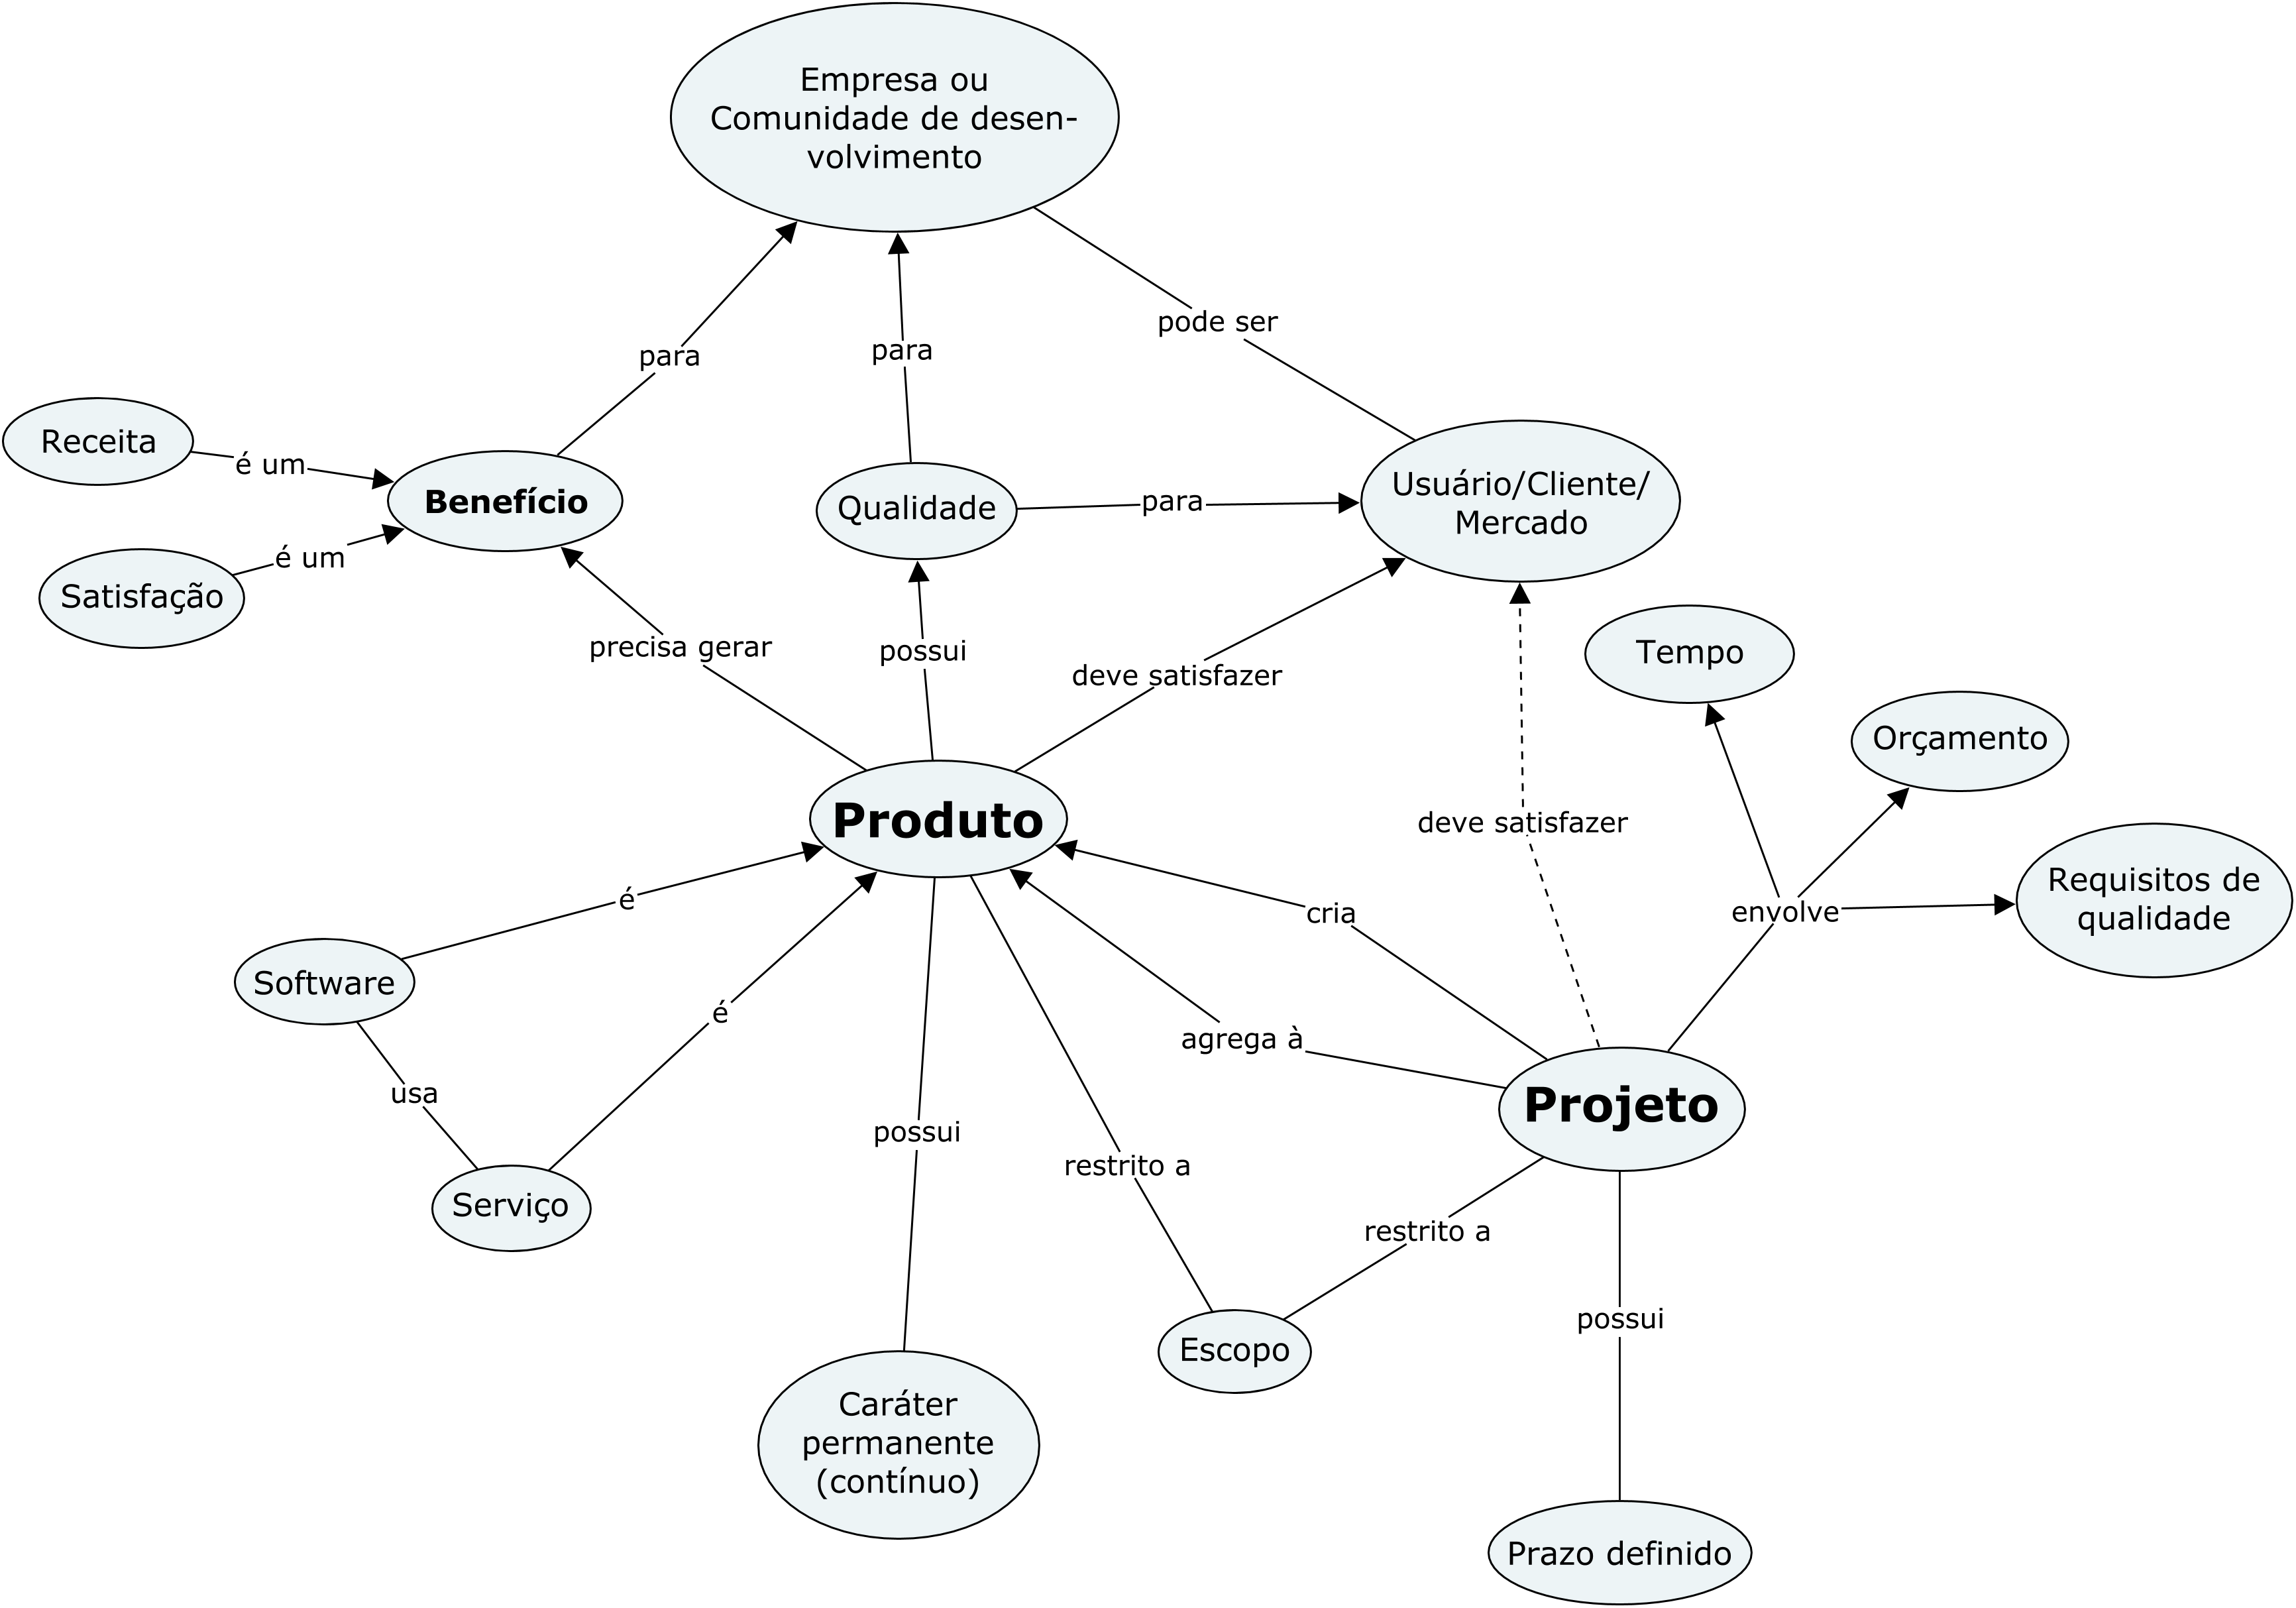
\includegraphics[width=\textwidth]{product}
	\end{center}
\end{frame}


\begin{frame}[parent={ie:agenda}, hasnext=false, hasprev=false]
	\frametitle{Produto}
	
	\begin{block:concept}{Definição}
		Um produto pode ser uma combinação de sistemas, soluções, materiais
		e serviços:
	
		\begin{itemize}
			\item Uma \textbf{solução} é produto específico para cliente
			criado a partir de diferentes produtos, processos e recursos,
			e ajustado para servir os propósitos específicos
			de negócio do cliente.
			
			\item Um \textbf{serviço} é um produto temporário e intangível que é
			resultante da cocriação de valor por ao menos uma atividade
			executada entre fornecedor e o cliente e que não implica em
			troca de propriedade.
		\end{itemize}
	\end{block:concept}
		
	\begin{block:fact}{}
		Produtos representam a essência do negócio, como ele prospera,
		cresce e traz lucros para a empresa.
		
		Projetos são o meio para derivar, entregar e suportar produtos
		e outros elementos de negócio relacionados a ele.
	\end{block:fact}
\end{frame}



\begin{frame}
	\frametitle{Produto}
	\framesubtitle{Produto de sucesso}

%	\begin{block:fact}{Sucesso de produto}
%		\begin{itemize}
%			\item Sucesso do projeto $\neq$ sucesso do produto
%			\item Entretanto, sucesso de projetos é condição para sucesso do produto.
%			\item Escopo e qualidade
%		\end{itemize}
%	\end{block:fact}
	
	\begin{block:ie}{Exemplos}
		\begin{itemize}
			\item Windows (sistema operacional): inicialmente um produto ruim, mas sucessivos projetos bem sucedidos tornaram-no em um produto de sucesso.
	
			\item Digg (agregador de notícias): inicialmente um bom produto, mas sucessivos projetos mal sucedidos levaram o produto à bancarrota.
		\end{itemize}

	\end{block:ie}
\end{frame}


% \begin{frame}
	\frametitle{Produto}
	
	\begin{center}
		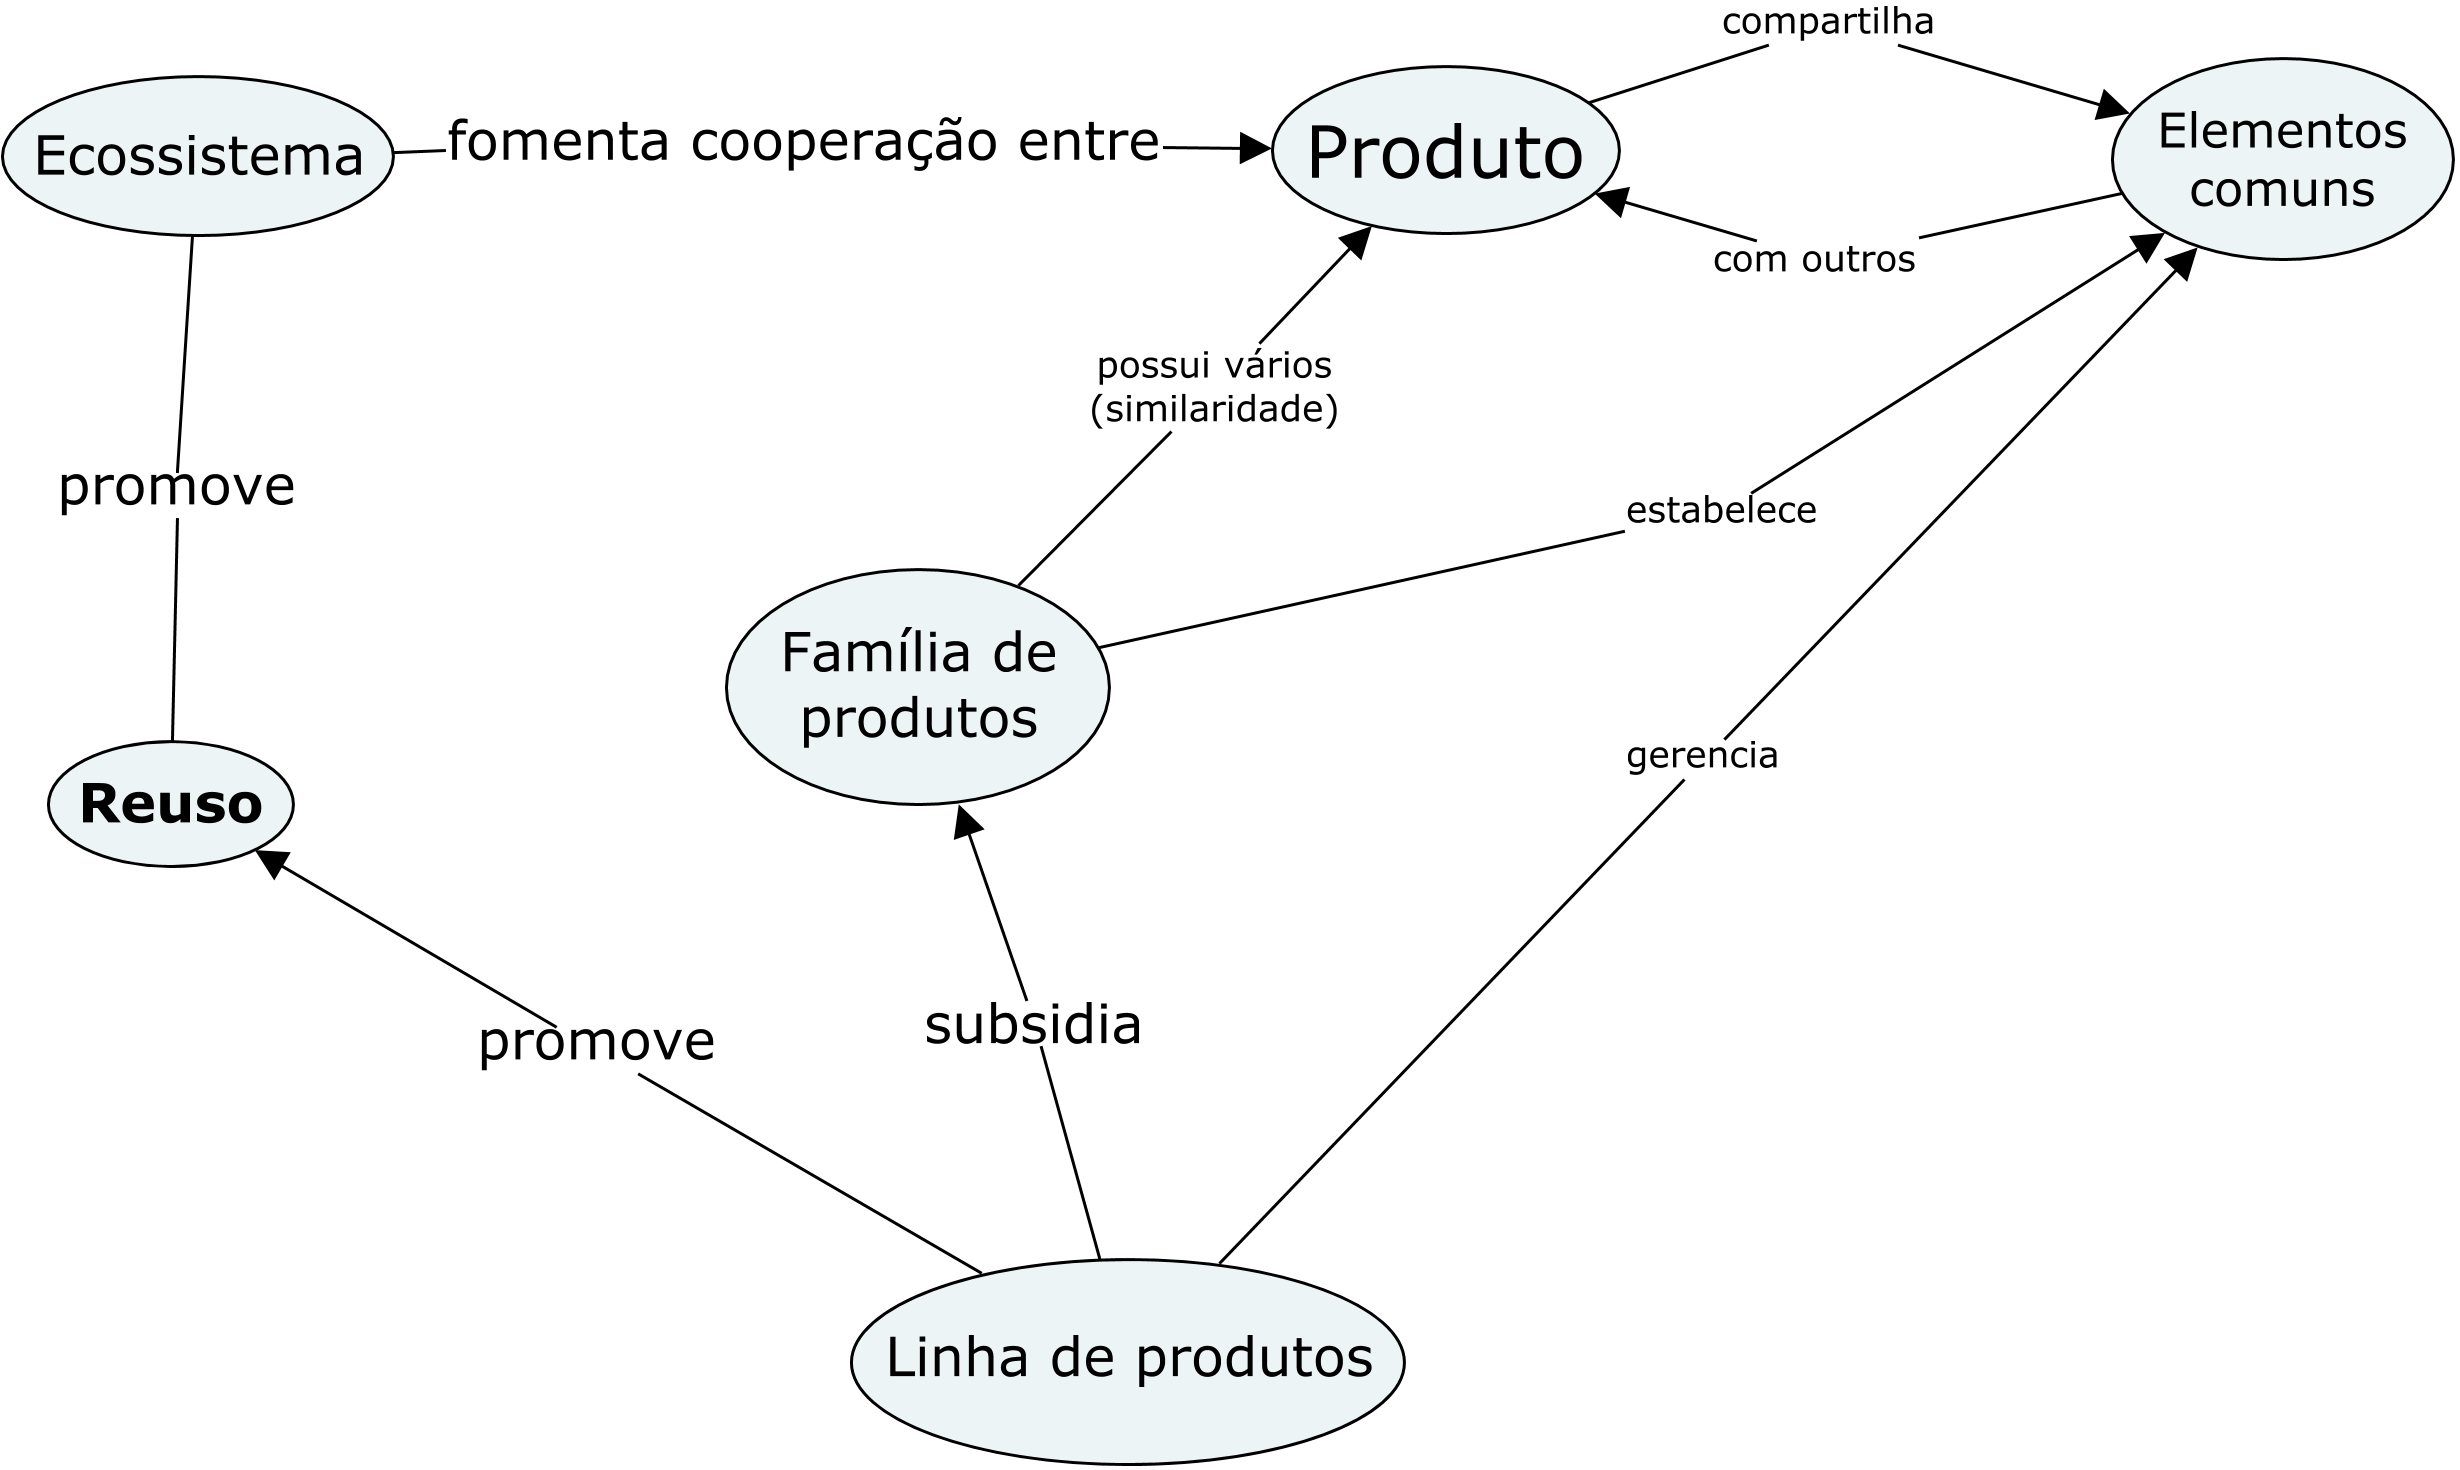
\includegraphics[width=\textwidth]{product-family-ecosystem}
	\end{center}
\end{frame}



\section{Gerenciamento}

\begin{frame}
	\frametitle{Gerenciamento de produto}

	\begin{block:concept}{Gerenciamento de produto}
		Gerenciamento de produto é a disciplina e o processo de negócio
		que governa o produto desde sua concepção para o mercado até sua
		entrega e retirada, trazendo o maior valor possível para o
		negócio da empresa.
	\end{block:concept}

	\begin{block:fact}{Principais grupos de processos}
		\begin{itemize}
			\item Gerenciamento de portfólio.
			\item Marketing do produto.
			\item Desenvolvimento do produto.
		\end{itemize}
	\end{block:fact}
	
	\note{
		\begin{itemize}
			\item Gerenciamento de produto bem sucedido significa a entrega do
			produto certo na hora certa para o mercado certo.
			
			\item Falar da experiência no NUMA: integração de aplicações técnicas (computação),
			gerenciamento (engenharia de produção) e negócio (relacionamento com clientes) no
			contexto de software livre.		
			
			\item Fazer o gancho para todas as atividades feitas e que constam no próximo slide.
		\end{itemize}
	}
\end{frame}



% \begin{frame}
% 	\frametitle{Gerenciamento de produto (software)}
% 	\framesubtitle{Produto X Projeto: Grupo de processos}
% 
% 	\begin{block:fact}{}
% 		\centering
% 		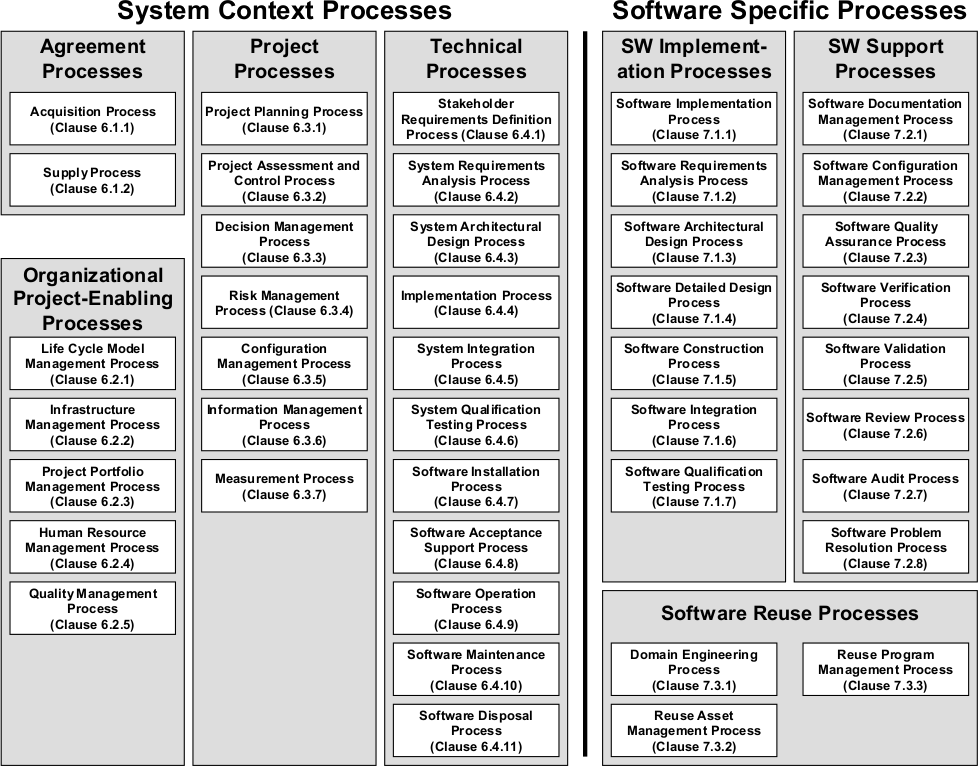
\includegraphics[width=\textwidth]{software-engineering/project-management/product/iso12207}
% 	\end{block:fact}
% 	
% 	\note{
% 		The ISO life cycle related standards for systems life cycle
% 		processes (ISO/IEC 15288:2002, 2002) and software life
% 		cycle processes (ISO/IEC 12207:1997, 1997) primarily look
% 		into the processes from analysis to development to distri-
% 		bution and further downstream towards operations and
% 		even disposal. They do not detail the upstream activities
% 		before project start or product launch.
% 	}
% \end{frame}

\begin{frame}
	\frametitle{Gerenciamento de produto (software)}

	\begin{block:fact}{\small Arcabouço de referência para gerenciamento de produtos (software)}
		\centering
		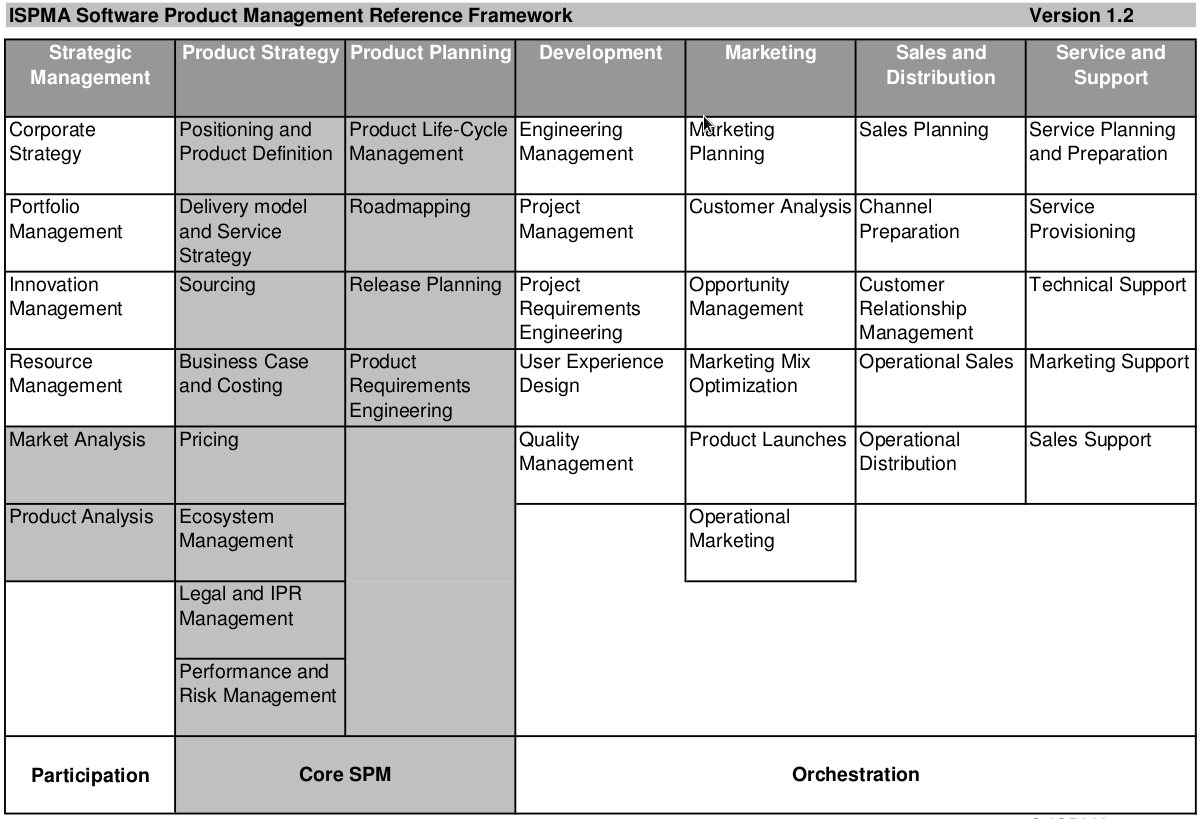
\includegraphics[width=\textwidth]{software-engineering/project-management/product/ispma}
	\end{block:fact}
	
	\note{
		\begin{itemize}  
			\item Market analysis and product analysis are the sources of the raw
			qualitative and quantitative decision-making data for the product manager.
		 
			\item Product strategy and product planning are the business-oriented core
			functions of product management.
		 
			\item The other functions (development, marketing, sales and
			distribution, support and services) are not directly related to the
			tasks of the product manager and thus he needs to collaborate
			with the respective departments about decisions concerning these
			functions.
		\end{itemize}
	}
\end{frame}


\subsection{Escopo}

\begin{frame}
	\frametitle{Gerenciamento de produto (software)}
	\framesubtitle{Escopo}
	
	\begin{block:concept}{Escopo}
		Definição de escopo é o processo de dividir objetivos ou requisitos
		de um produto e de um projeto em partes menores e mais concisas.
	\end{block:concept}


	\begin{block:fact}{Escopo}
		\begin{center}
			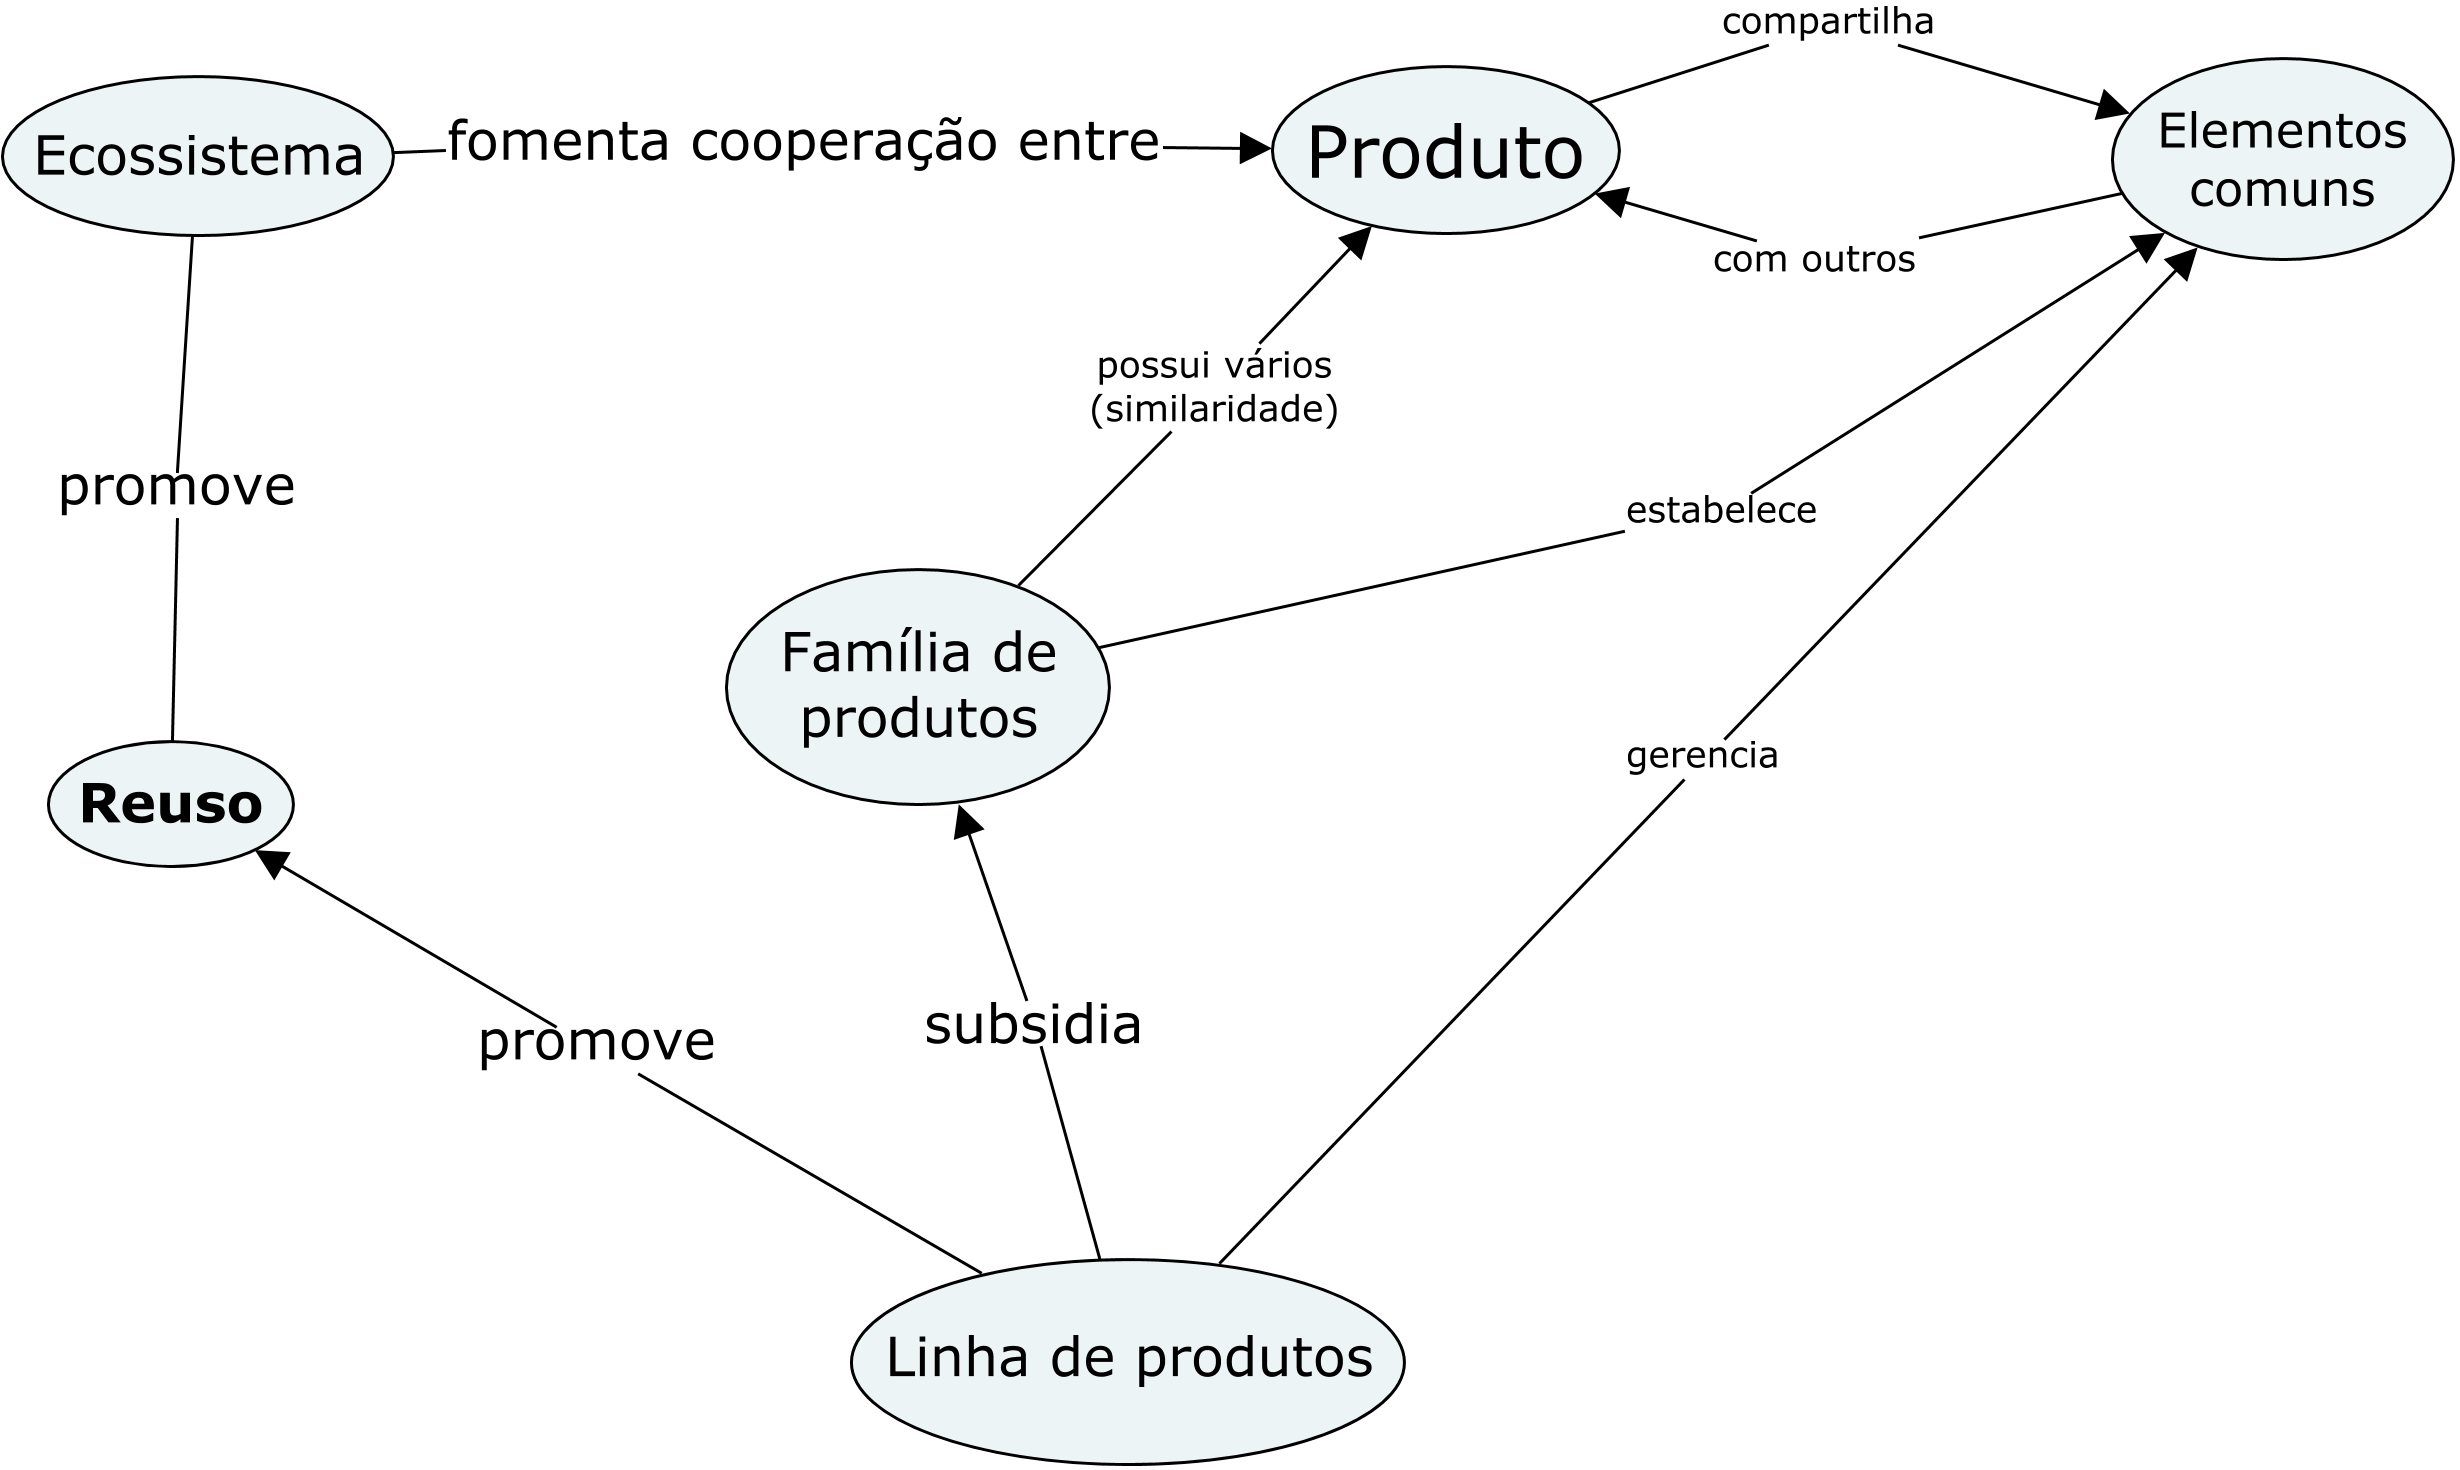
\includegraphics[width=.8\textwidth]{product-family-ecosystem}
		\end{center}
	\end{block:fact}
	
	\note{
		Breve história de evolução:
		\begin{itemize}
			\item Primeiros sistemas computacionais: software + hardware, totalmente integrados.
			
			\item IBM + MS-DOS
			
			\item Windows
			
			\item Web (mashups, serviços Web)
			
			\item Aplicações para dispositivos móveis (appstores)
		\end{itemize}
		
		Escopo cada vez mais reduzido, o que também proporciona a definição de mais produtos e projetos!
		
		Ecossistemas: preocupação em oferecer bons serviços comuns a diversas aplicações diferentes.
	}
\end{frame}


\begin{frame}
	\frametitle{Gerenciamento de produto (software)}
	\framesubtitle{Escopo: Produto X Projeto}
	
	\begin{block:fact}{Escopo do \textbf{produto}}
		\begin{itemize}
			\item Tendências de mercado
			\item Requisitos de cliente
			\item Interesses da empresa ou comunidade (lucro, aumento de participação/visibilidade)
		\end{itemize}
	\end{block:fact}
	
	\begin{block:fact}{Escopo do \textbf{projeto}}
		\begin{itemize}
		 	\item Entrega do projeto na data correta,
		 	
		 	\item Cumprimento do orçamento estabelecido.
		 	
		 	\item Satisfação de requisitos de qualidade.
		\end{itemize}
	\end{block:fact}

	\note{
		\begin{itemize}
			\item Produto: voltado para o lançamento e criação.
			
			\item Projeto: voltado o desenvolvimento, manutenção.
			
			\item Atualmente é possível uma relação quase 1 para 1 entre produto e projeto em alguns segmentos,
			ou seja, lançar um produto distinto a cada projeto.
		\end{itemize}
	}
\end{frame}


\subsection{Proteção intelectual}


\begin{frame}
	\frametitle{Proteção intelectual}
	
	\note{
		Gestão das propriedades intelectuais:
		\begin{itemize}
			\item Quais são? Direitos autorais (copyright), segredo industrial e patentes. Explicar
			\item Licença de software: proprietário e software livre.
			\item Gerenciamento da proteção intelectual e os desafios: Oracle X Google (Google protegendo seu ecosistema)
		\end{itemize}
	}
\end{frame}



\subsection{Planejamento de lançamentos}

\begin{frame}
	\frametitle{Planejamento do lançamento de versões do produto}
	
	\begin{center}
		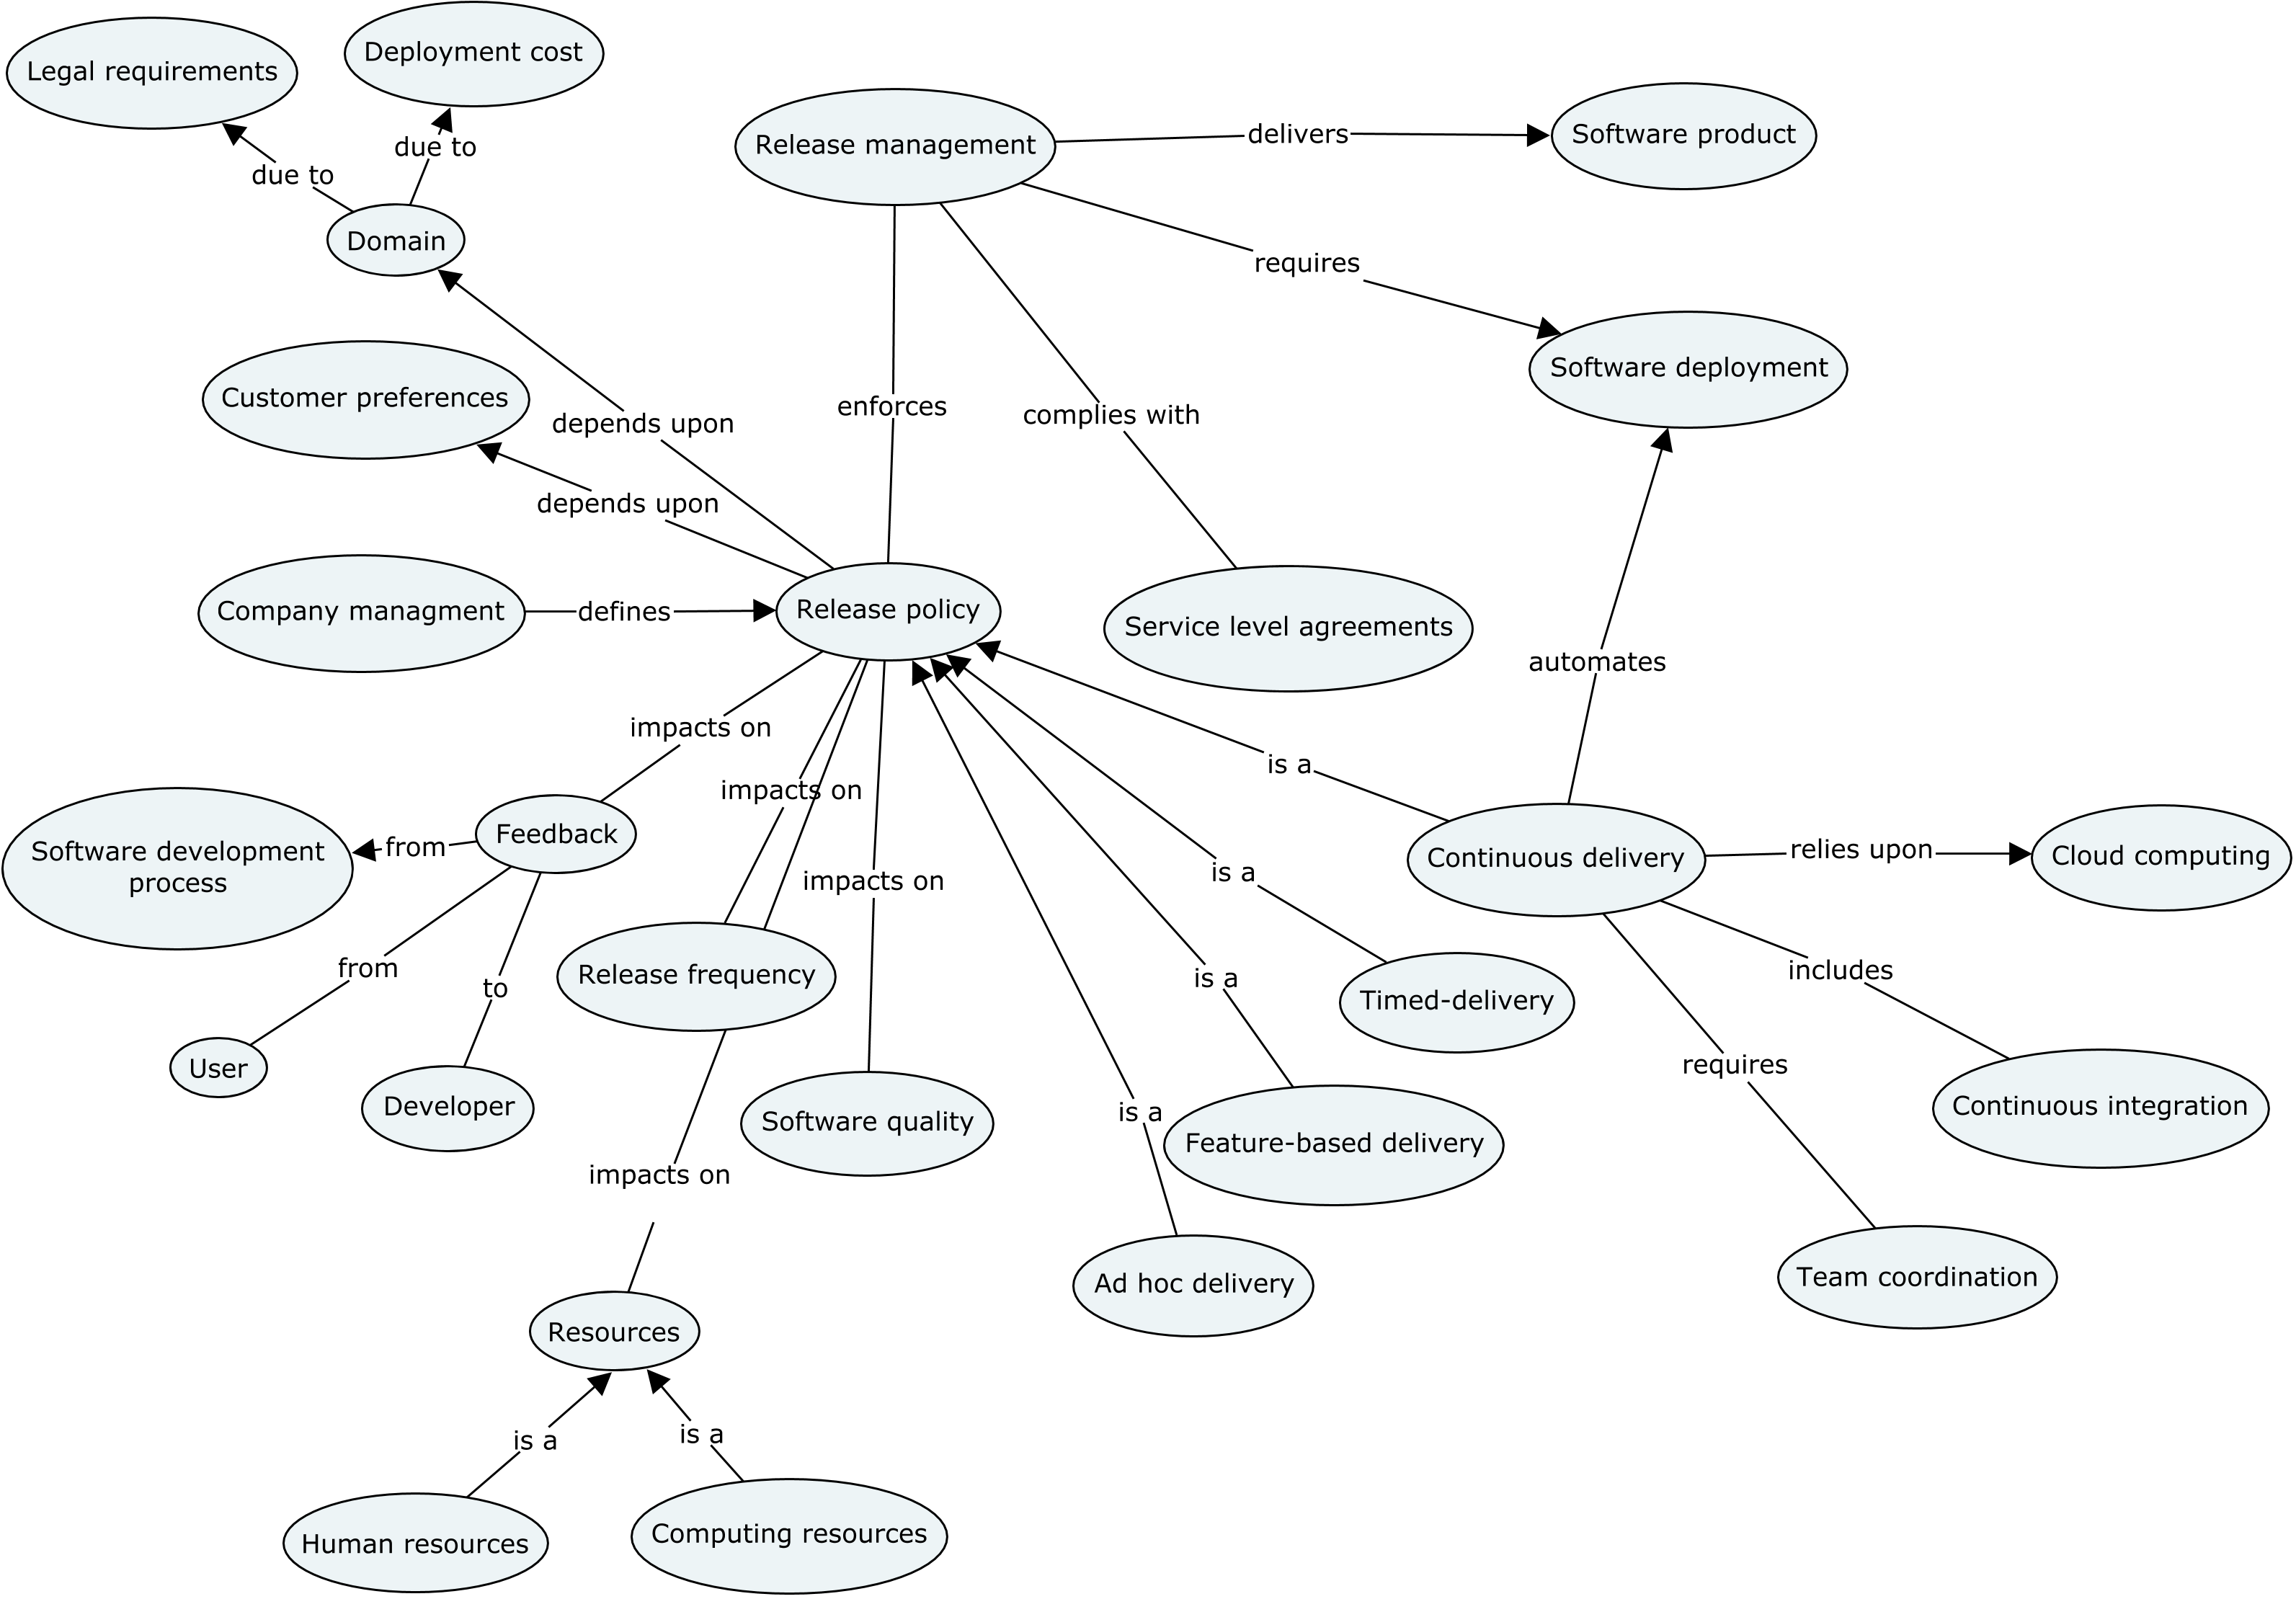
\includegraphics[width=\textwidth]{release-management}
	\end{center}
	
	\note{
		\begin{itemize}
			\item Flowing releases (lançamentos contínuos)
			\item Versões timeboxed (Ubuntu, Fedora)
			\item Atualizações constantes e ubíquas
		\end{itemize}
	}
\end{frame}



\subsection{Comunidade de desenvolvimento (OSS)}

\begin{frame}
	\frametitle{OSS}
	
	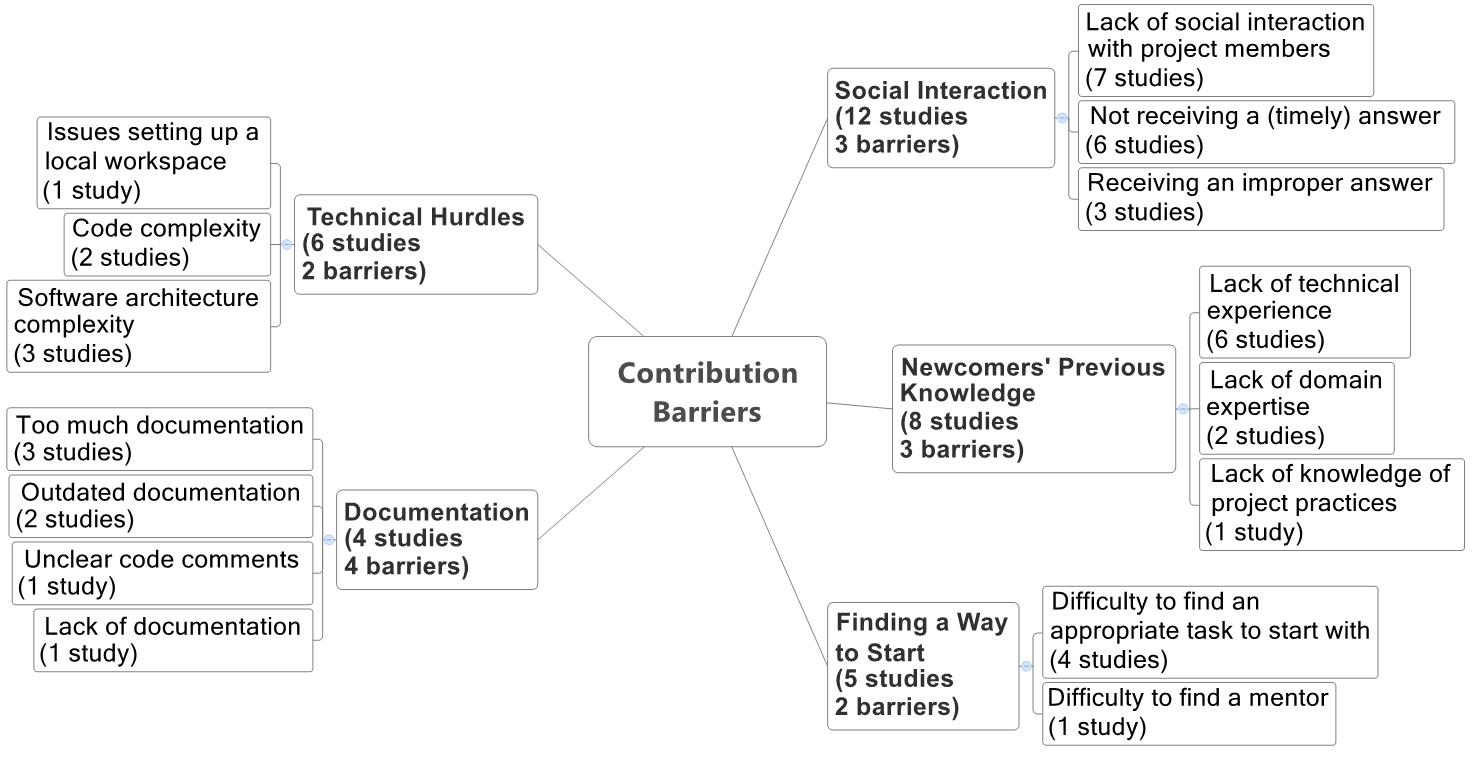
\includegraphics[width=\textwidth]{Barriers4}
	
	\note{O ``projeto de software livre'' (que, na realidade, é um produto, precisa apoiar a comunidade que o mantém.)}
\end{frame}

\subsection{Qualidade de produto}
\begin{frame}[parent={ie:agenda}, hasnext=false, hasprev=false]
	\frametitle{Qualidade de produto}
	
	\begin{block:concept}{Qualidade de produto}
		Qualidade é a totalidade de características e critérios de um produto ou
		serviço que exercem suas habilidades para satisfazer as necessidades 
		declaradas ou envolvidas.
	\end{block:concept}
	
	\begin{block:fact}{}
		Embora seja difícil definir exatamente qualidade (em termos de satisfação
		de propriedades), é fácil reconhecer produtos de boa qualidade.
	\end{block:fact}
\end{frame}


\begin{frame}[hasnext=true, hasprev=true]
	\frametitle{Qualidade de produto}
	
	\begin{block:fact}{Qualidade de produto e processo}
		\centering
		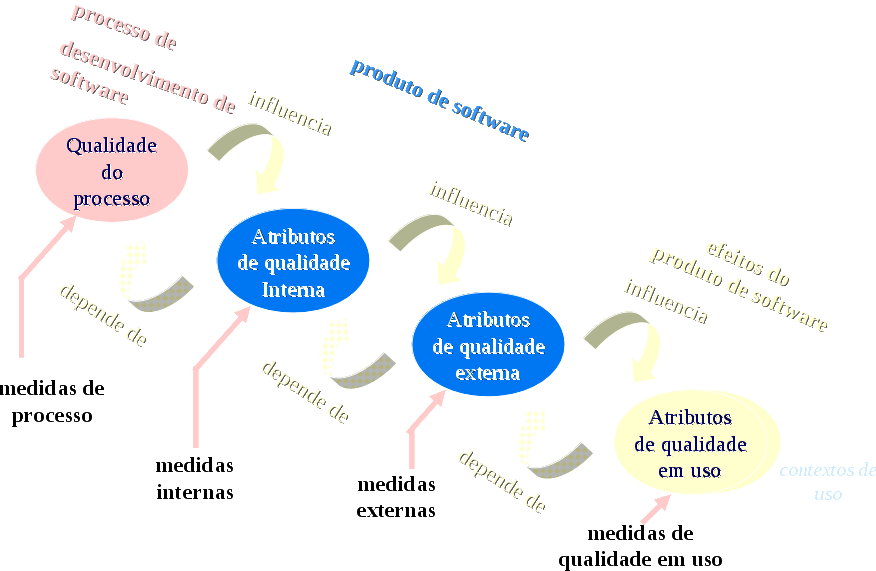
\includegraphics[width=\textwidth]{software-engineering/project-management/product/product-quality}
	\end{block:fact}
	
	\begin{block:fact}{}
		A avaliação de produtos de software tem sido uma das formas empregadas por
		organizações que produzem ou adquirem software para obtenção de maior
		qualidade nesses produtos, sejam eles produtos completos ou partes a serem
		integradas num sistema computacional mais amplo.
	\end{block:fact}
\end{frame}


\begin{frame}
	\frametitle{Qualidade de produto}
	
	\begin{block:fact}{Perspectivas}
		\centering
		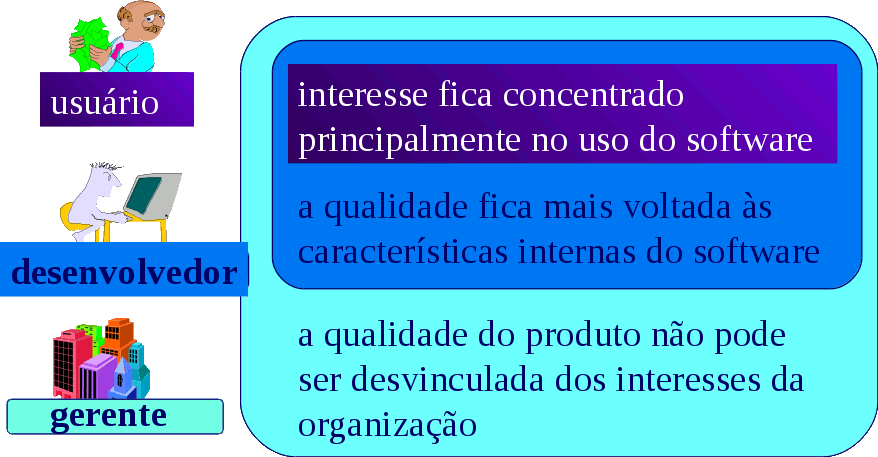
\includegraphics[width=\textwidth]{software-engineering/project-management/product/product-quality-perspectives}
	\end{block:fact}
\end{frame}


\begin{frame}
	\frametitle{Qualidade de produto}
	\framesubtitle{Modelos de qualidade}
	
	\begin{block:fact}{Modelos de qualidade de produto}
		\begin{itemize}
			\item Modelo de McCall
			\item Modelo de qualidade da ISO 9126
			\item Modelo de Dromey
			\item Modelo da 25010
		\end{itemize}
	\end{block:fact}
\end{frame}




\subsubsection{McCall}
\begin{frame}[parent={ie:agenda}, hasnext=false, hasprev=false]
	\frametitle{Modelo de McCall}

	\begin{block:concept}{Modelo de McCall}
		\begin{itemize}
			\item Desenvolvido para a Força Aérea Norte-Americana
			\item Organizado em:
			\begin{itemize}
				\item Fatores: visão externa do software (usuários).
				\item Critérios: visão interna do software (desenvolvedores).
				\item Métricas
			\end{itemize}
		\end{itemize}
	\end{block:concept}
\end{frame}


\begin{frame}[hasnext=true, hasprev=true]
	\frametitle{Modelo de McCall}

	\begin{block:fact}{Pontos de vista}
		Fatores e critérios relacionados a três pontos de vista:
		\begin{itemize}
			\item Operação/uso do produto;
			\item Revisão/mudança do produto;
			\item Transição do produto.
		\end{itemize}
	\end{block:fact}
\end{frame}


\begin{frame}
	\frametitle{Modelo de McCall}
	\framesubtitle{Fatores: Operação}

	\begin{block:concept}{Modelo de McCall}
		\centering
		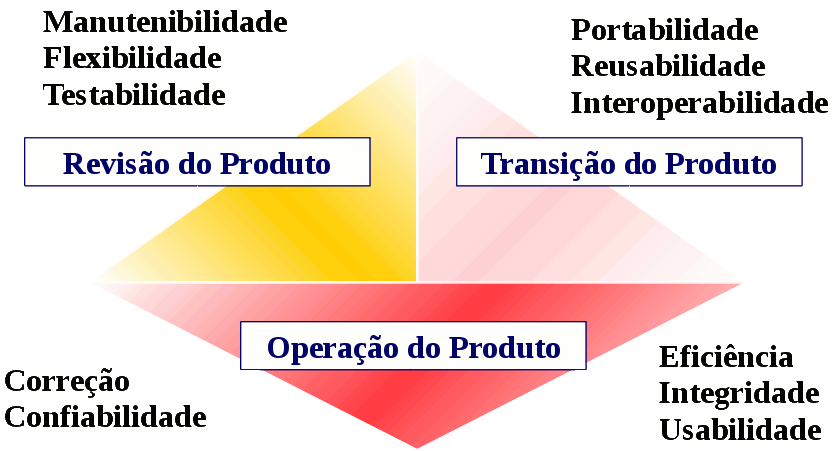
\includegraphics[width=.7\textwidth]{software-engineering/project-management/product/mccall/mccall}
	\end{block:concept}
\end{frame}


\begin{frame}
	\frametitle{Modelo de McCall}
	\framesubtitle{Fatores: Operação}
	
	\begin{block:concept}{Fatores de operação}
		\begin{itemize}
			\item \textbf{Correção}: Quanto um programa satisfaz sua especificação e cumpre os
			objetivos visados pelo cliente.
			\item \textbf{Confiabilidade}: Quanto que se pode esperar que um programa execute a
			função pretendida com a precisão exigida.
			\item \textbf{Eficiência}: Quantidade de recursos de computação e de código exigida
			para que um programa execute sua função.
			\item \textbf{Integridade}: Quanto o acesso ao software ou a dados, por pessoas
			não-autorizadas, pode ser controlado.
			\item \textbf{Usabilidade}: O esforço para aprender, operar, preparar a entrada e
			interpretar a saída de um programa.
		\end{itemize}
	\end{block:concept}
\end{frame}

\begin{frame}
	\frametitle{Modelo de McCall}
	\framesubtitle{Fatores: Revisão}

	\begin{block:concept}{Fatores de Revisão}
		\begin{itemize}
			\item \textbf{Manutenibilidade}: O esforço exigido para localizar e reparar erros
			em um programa.
			\item \textbf{Flexibilidade}: O esforço exigido para modificar um programa
			operacional.
			\item \textbf{Testabilidade}: O esforço exigido para testar um programa a fim de
			garantir que ele execute a função pretendida.
		\end{itemize}
	\end{block:concept}
\end{frame}


\begin{frame}
	\frametitle{Modelo de McCall}
	\framesubtitle{Fatores: Transição}

	\begin{block:concept}{Fatores de Transição}
		\begin{itemize}
			\item \textbf{Portabilidade}: O esforço exigido para transferir o programa de um
			ambiente de sistema de hardware e/ou software para outro.
			\item \textbf{Reusabilidade}: Quanto um programa (ou partes de um programa) pode 
			ser reutilizado em outras aplicações.
			\item \textbf{Interoperabilidade}: O esforço exigido para acoplar um sistema a
			outro.
		\end{itemize}
	\end{block:concept}
\end{frame}

\begin{frame}
	\frametitle{Modelo de McCall}
	\framesubtitle{Métricas}

	\begin{block:fact}{Atributos de qualidade medidos}
		\begin{columns}
			\column{.45\textwidth}
			\begin{itemize}
				\item Auditabilidade
				\item Acurácia
				\item Comunidade de Comunicação
				\item Inteireza
				\item Concisão
				\item Consistência
				\item Comunidade de Dados
				\item Tolerância a Erros
				\item Eficiência de Execução
				\item Expansabilidade
				\item Generalidade
			\end{itemize}
			
			\column{.45\textwidth}
			\begin{itemize}
				\item Independência de Hardware
				\item Instrumentação
				\item Modularidade
				\item Operabilidade
				\item Segurança
				\item Autodocumentação
				\item Simplicidade
				\item Independência de Software Básico
				\item Rastreabilidade
				\item Treinamento
			\end{itemize}
		\end{columns}
	\end{block:fact}
	
	\note{
		\begin{itemize}
			\item Auditabilidade - facilidade com que se pode checar a conformidade aos padrões.
			\item Acurácia - A precisão das computações e do controle.
			\item Comunidade de Comunicacão (Communication Commonality) - O grau em que as interfaces padrões, protocolos e larguras de banda (bandwidths) são usados.
			\item Inteireza - O quanto a implementação total da função requerida foi conseguida.
			\item Eficiência de Execução - O desempenho de run-time de um programa.
			\item Expansabilidade - O quanto o projeto arquitetural, procedimental e de dados podem ser ampliados.
			\item \ldots
			\item Generalidade - A amplitude de aplicação em potencial de componentes de programa.
			\item Modularidade - A independência funcional dos componentes do programa.
			\item Operabilidade - A facilidade de operação de um programa.
			\item Segurança - A disponibilidade de mecanismos que controlem ou protejam programas e dados.
			\item Autodocumentação - O quanto o código-fonte apresenta documentação significativa.
			\item Simplicidade - O quanto um programa pode ser entendido sem dificuldade.
			\item Independência do Software Básico - O quanto um programa é independente de particularidades não padronizadas de linguagens de programação non-standard, das características de sistemas operacionais e de outras sujeições ambientais.
			\item Rastreabilidade - A capacidade de rastrear uma representação de projeto ou componente de programa até os requisitos.
			\item Treinamento - O quanto o software auxilia no sentido de ajudar novos usuários a aplicarem o sistema.
			\item Independência de Hardware - O quanto o software é desvinculado do hardware em que opera.
			\item Instrumentação - O quanto o programa monitora sua própria operação e identifica erros que venham a ocorrer.
		\end{itemize}
	}
\end{frame}


\begin{frame}
	\frametitle{Modelo de McCall}
	\framesubtitle{Fatores e Métricas}

	\begin{block:fact}{``Métricas''}
		Define-se conjunto de medições para desenvolver expressões que poderão ser
		utilizadas para avaliar cada um dos fatores.
	\end{block:fact}
	
	\begin{block:fact}{}
		$F_q = \sum_{1}^m c_n \cdot m_n$, em que:
		\begin{itemize}
		 \item $F_q$ = fator de qualidade de software
		 \item $c_n$ = coeficiente de regressão
		 \item $m_n$ = métrica que afeta o fator de qualidade
		\end{itemize}
	\end{block:fact}
	
	\begin{block:fact}{}
		Total de fatores: 11
	
		Valores para $m_n$ são obtidos a partir de checklists, sendo graduados em
		0 a 10.
	\end{block:fact}
\end{frame}



\begin{frame}
	\frametitle{Modelo de McCall}
	\framesubtitle{Fatores e Métricas}

	\begin{block:fact}{}
		$F_q = \sum_{1}^m c_n \cdot m_n$
	\end{block:fact}

	\begin{block:fact}{}
		\centering
		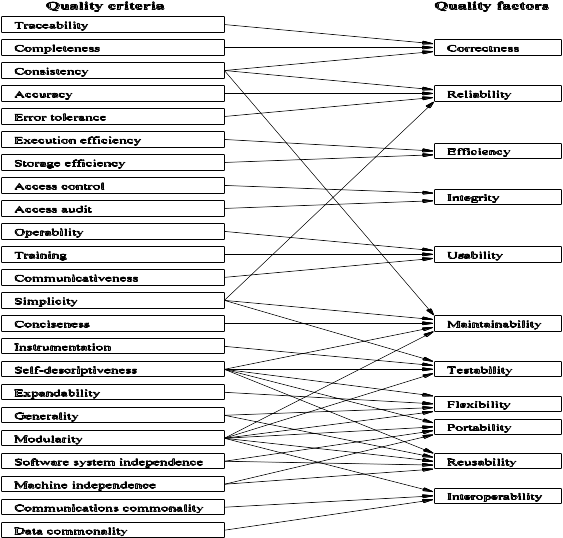
\includegraphics[width=.7\textwidth]{software-engineering/project-management/product/mccall/mccall-factor_metrics}
	\end{block:fact}
\end{frame}



\subsubsection{ISO 9126}
\begin{frame}[parent={ie:agenda}, hasnext=true, hasprev=false]
	\frametitle{ISO 9126}

	\begin{block:concept}{ISO 9126}
		Conjunto de normas ISO/IEC sobre a qualidade de produto de software.
	\end{block:concept}
	
	\begin{block:fact}{Partes da norma}
		\begin{itemize}
			\item ISO/IEC 9126-1: Modelo de qualidade.
			\item ISO/IEC 9126-2: Métricas externas.
			\item ISO/IEC 9126-3: Métricas internas.
			\item ISO/IEC 9126-4: Métricas de qualidade em uso.
		\end{itemize}
	\end{block:fact}

	\begin{block:fact}{AVISO}
		A coleção de norma ISO 9126 foi aposentada/substituída pela coleção
		da ISO 25000!
	\end{block:fact}
	
	\note{
		\begin{itemize}
			\item Primeiros esforços para padronização: 1978
			\item Início de desenvolvimento da norma: 1985
			\begin{itemize}
				\item Information Technology -- Software product evaluation -- Quality
				characteristics and guidelines for their use
			\end{itemize}
			\item Publicada em 1991
			\item Atualizada em 2001
			\begin{itemize}
				\item Software Engineering -- Product Quality
			\end{itemize}
			\item ``Aposentada'' em 2008 pela ISO 25000
		\end{itemize}
	}
\end{frame}


\begin{frame}[hasnext=false, hasprev=true]
	\frametitle{ISO 9126}
	\framesubtitle{ISO 9126-1: Modelo de qualidade}
	
	\begin{block:fact}{Modelo de qualidade}
		Organizada em características, subcaracterísticas e métricas.
	\end{block:fact}
	
	\begin{block:fact}{}
		Modelo organizado hierarquicamente por características e subcaracterísticas.
		\begin{itemize}
			\item 6 características
			\item 27 subcaracterísticas
			\item ao menos uma métrica por característica
		\end{itemize}
	\end{block:fact}
\end{frame}


\begin{frame}
	\frametitle{ISO 9126-1: Modelo de qualidade}
	\framesubtitle{Características}
	
	\begin{block:fact}{Características}
		\begin{itemize}
			\item Funcionalidade
			\item Confiabilidade
			\item Usabilidade
			\item Eficiência
			\item Manutenibilidade
			\item Portabilidade
		\end{itemize}
	\end{block:fact}

	\begin{block:fact}{}
		\begin{itemize}
			\item \textbf{O que?} Funcionalidade
			\item\textbf{ Quando e como?} Confiabilidade, usabilidade, eficiência,
			manutenibilidade e portabilidade.
		\end{itemize}
	\end{block:fact}
\end{frame}


\begin{frame}
	\frametitle{ISO 9126-1: Modelo de qualidade}
	\framesubtitle{Características}
	
	\begin{block:fact}{Funcionalidade}
		Conjunto de atributos que evidenciam a existência de um conjunto de funções
		e suas propriedades especificadas.

		Funções: aquilo que satisfaz as necessidades implícitas e explícitas
		(requisitos funcionais)
	\end{block:fact}
	
	\begin{block:fact}{Subcaracterísticas}
		\begin{itemize}
			\item Adequação: propõe-se a fazer o que é apropriado?
			\item Acurácia: faz o que foi proposto de forma correta?
			\item Interoperabilidade: é capaz de interagir com os sistemas especificados?
			\item Segurança de acesso: evita acesso não autorizado a programas e dados?
			\item Conformidade: está de acordo com normas técnicas e aspectos legais
			relacionados à funcionalidade?
		\end{itemize}
	\end{block:fact}
\end{frame}



\begin{frame}
	\frametitle{ISO 9126-1: Modelo de qualidade}
	\framesubtitle{Características}
	
	\begin{block:fact}{Confiabilidade}
		Conjunto de atributos que evidenciam a capacidade do software manter seu nível
		de desempenho sob condições estabelecidas durante um período de tempo
		estabelecido.
	\end{block:fact}
	
	\begin{block:fact}{Subcaracterísticas}
		\begin{itemize}
			\item Maturidade: com que frequência apresenta defeitos?
			\item Tolerância a falhas: Na ocorrência de um erro, como o sistema
			reage? Ocorre uma falha?
			\item Recuperabilidade: O produto é capaz de se recuperar em casos de
			falhas?
			\item Conformidade
		\end{itemize}
	\end{block:fact}
\end{frame}



\begin{frame}
	\frametitle{ISO 9126-1: Modelo de qualidade}
	\framesubtitle{Características}
	
	\begin{block:fact}{Usabilidade}
		Conjunto de atributos que evidenciam o esforço necessário para utilizar o
		software bem como para o julgamento individual deste uso.
	\end{block:fact}
	
	\begin{block:fact}{Subcaracterísticas}
		\begin{itemize}
			\item Inteligibidade: É fácil entender o conceito da aplicação e sua
			aplicabilidade?
			\item Apreensibilidade: É fácil aprender a usar?
			\item Operabilidade: É fácil de operar e controlar?
			\item Atratividade: É atrativa ao usuário?
			\item Conformidade
		\end{itemize}
	\end{block:fact}
\end{frame}


\begin{frame}
	\frametitle{ISO 9126-1: Modelo de qualidade}
	\framesubtitle{Características}
	
	\begin{block:fact}{Eficiência}
		Conjunto de atributos que evidenciam o relacionamento entre o nível de
		desempenho do software e quantidade de recursos usados sob condições
		previamente estabelecidas.
	\end{block:fact}
	
	\begin{block:fact}{Subcaracterísticas}
		\begin{itemize}
			\item Comportamento em relação ao tempo
			\item Comportamento em relação aos custos
			\item Conformidade
		\end{itemize}
	\end{block:fact}
\end{frame}


\begin{frame}
	\frametitle{ISO 9126-1: Modelo de qualidade}
	\framesubtitle{Características}
	
	\begin{block:fact}{Manutenibilidade}
		Conjunto de atributos que evidenciam o esforço necessário para fazer
		modificações no software.
	\end{block:fact}
	
	\begin{block:fact}{Subcaracterísticas}
		\begin{itemize}
			\item Analisabilidade: é fácil encontrar um defeito quando detectada uma falha?
			\item Modificabilidade: É fácil modificar e adaptar o software?
			\item Estabilidade: Existe risco de efeitos inesperados quando realizadas alterações?
			\item Testabilidade: É fácil validar o software modificado?
			\item Conformidade
		\end{itemize}
	\end{block:fact}
\end{frame}


\begin{frame}
	\frametitle{ISO 9126-1: Modelo de qualidade}
	\framesubtitle{Características}
	
	\begin{block:fact}{Portabilidade}
		Conjunto de atributos que evidenciam a capacidade do software ser transferido
		de um ambiente para outro.
	\end{block:fact}
	
	\begin{block:fact}{Subcaracterísticas}
		\begin{itemize}
			\item Adaptabilidade: É fácil adaptar para ambientes diferentes?
			\item Instalação: É fácil de instalar?
			\item Capacidade de ser substituído: É fácil substituir este software por outro?
			\item Coexistência: Pode coexistir com outros produtos e compartilhar os recursos?
			\item Conformidade
		\end{itemize}
	\end{block:fact}
\end{frame}


\begin{frame}
	\frametitle{ISO 9126-1: Modelo de qualidade}
	\framesubtitle{Métricas internas e externas}
	
	\begin{block:fact}{Subcaracterísticas e métricas}
		Subcaracterísticas são medidas por métricas internas e externas.
		\begin{itemize}
			 \item Métricas externas: exemplificadas na ISO/IEC 9126-2
			 \item Métricas internas: exemplificadas na ISO/IEC 9126-3
		\end{itemize}
	\end{block:fact}
	
	\begin{block:concept}{Métrica interna}
	Aplicável aos artefatos de software (durante o desenvolvimento)
	\end{block:concept}

	\begin{block:concept}{Métrica externa}
	Aplicável ao produto de software durante a fase de teste (aplicada pelo
	desenvolvedor, mas com o ponto de vista do usuário)
	\end{block:concept}
\end{frame}



\begin{frame}
	\frametitle{ISO 9126}
	\framesubtitle{Qualidade em uso}
	
	\begin{block:fact}{Qualidade em uso}
		Refere-se ao uso do software em ambiente específico e não às propriedades
		do software.
	\end{block:fact}
\end{frame}


\begin{frame}
	\frametitle{ISO 9126}
	\framesubtitle{Qualidade em uso}
	
	\begin{block:fact}{Características}
		\begin{itemize}
			\item Eficácia
			\begin{itemize}
				\item Permite que o usuário atinja metas com acurácia e completitude
			\end{itemize}
			
			\item Produtividade
			\begin{itemize}
				\item Permite que o usuário utilize quantidade apropriada de recursos
			\end{itemize}

			\item Segurança
			\begin{itemize}
				\item Apresentar níveis aceitáveis de risco a pessoas, negócio, propriedade e ambiente
			\end{itemize}

			\item Satisfação
			\begin{itemize}
				\item Satisfaz o usuário
			\end{itemize}
		\end{itemize}
	\end{block:fact}
\end{frame}

\begin{frame}
	\frametitle{ISO 9126}
	\framesubtitle{Qualidade em uso}
	
	\begin{block:fact}{Métricas}
		Exemplificadas na ISO/IEC 9126-4.
	\end{block:fact}
\end{frame}


\begin{frame}
	\frametitle{ISO 9126}
	\framesubtitle{Limitações}
	
	\begin{block:fact}{Limitações}
		\begin{itemize}
			\item Falta de evidências para a criação da norma
			\begin{itemize}
				\item Não foram executados estudos experimentais para avaliar as
				características e subcaracterísticas
			\end{itemize}
			
			\item Difícil aplicação
			\begin{itemize}
				\item Falta de diretivas (\foreign{guidelines})
				\item ``Genérica demais''
			\end{itemize}
		\end{itemize}
	\end{block:fact}
\end{frame}

\begin{frame}
	\frametitle{ISO 9126}
	\framesubtitle{Limitações}
	
	\begin{block:fact}{Measuring software product quality: a survey of ISO/IEC 9126 (Jung et al.)}
		\begin{itemize}
			\item Qualidade é um vetor (dimensões são as características de qualidade).

			\item Fatores analisados: todos menos as características de confiabilidade
			e todas as subcaracterísticas sobre conformidade.
			
			\item Cada questionário avaliou o mesmo produto quanto às subcaracterísticas
			da norma.
			
			\item PCA para identificar se os fatores realmente caracterizam uma
			dimensão (correlação entre as subcaracterísticas quanto à qualidade do
			produto).
		\end{itemize}
	\end{block:fact}
\end{frame}


\begin{frame}
	\frametitle{ISO 9126}
	\framesubtitle{Limitações}
	
	\begin{block:fact}{Measuring software product quality: a survey of ISO/IEC 9126 (Jung et al.)}
		\centering
		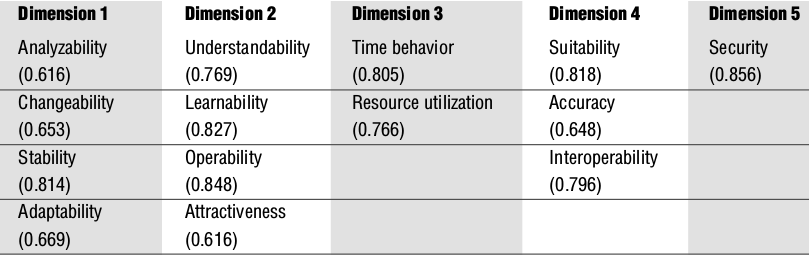
\includegraphics[width=\textwidth]{software-engineering/project-management/product/iso9126/jung-etal}
	\end{block:fact}
	
	\note{
		\begin{itemize}
			\item Quatro subcaracterísticas não estão presentes (correlação inferior a
			0,6): testabilidade, instalabilidade, substituibilidade, coexistência)
			
			\item Primeira dimensão não é consistente (adaptabilidade)
			
			\item Segurança não está correlacionada com outras características
		\end{itemize}
	}
\end{frame}

%
%
%\begin{frame}
%	\frametitle{ISO 9126}
%	\framesubtitle{Limitações}
%	
%	\begin{block:fact}{The use and usefulness of the ISO/IEC 9126 quality standard (Al-Kilidar et al.)}
%		\begin{itemize}
%			\item Avaliação de produto com a ISO/IEC 9126 por alunos de graduação
%			\begin{itemize}
%				\item Avaliação do projeto (design) de um produto
%			\end{itemize}
%			
%			\item Conclusão: norma é inútil
%		\end{itemize}
%	\end{block:fact}
%\end{frame}
%
%
%\begin{frame}
%	\frametitle{ISO 9126}
%	\framesubtitle{Limitações}
%	
%	\begin{block:fact}{The use and usefulness of the ISO/IEC 9126 quality standard (Al-Kilidar et al.)}
%		Limitações do estudo:
%		\begin{itemize}
%			\item Avaliaram artefato ``design'', não o produto
%			\item Não utilizaram um processo de avaliação
%			\begin{itemize}
%				\item Não definiram métricas (norma apenas \textbf{sugere} métricas)
%				\item Não treinaram avaliações antes de executar o experimento
%			\end{itemize}
%		\end{itemize}
%	\end{block:fact}
%\end{frame}
%
%
%\begin{frame}
%	\frametitle{ISO 9126}
%	\framesubtitle{Limitações}
%	
%	\begin{block:fact}{The use and usefulness of the ISO/IEC 9126 quality standard (Al-Kilidar et al.)}
%		Resultados úteis do estudo:
%		\begin{itemize}
%			\item Norma realmente possui problemas quanto a definições de termos
%			
%			\item Hierarquização das características/subcaracterísticas e seleção de
%			métricas
%			\begin{itemize}
%				\item Métrica útil para mais de uma subcaracterística
%				\item Isso não é vedado pela norma, mas ela passa a impressão de que sim
%			\end{itemize}
%			
%			\item Não são especificados requisitos para os dados coletados
%		\end{itemize}
%	\end{block:fact}
%\end{frame}

% \subsubsection{Dromey}
% \begin{frame}[parent={ie:agenda}, hasnext=true, hasprev=false]
	\frametitle{Dromey}

	\begin{block:concept}{Modelo de Dromey}
		Qualidade definida pela avaliação de propriedades de qualidade quanto às
		características do produto
		\begin{itemize}
			\item Produto organizado em componentes (\foreign{structural form})
			
			\item Avaliação a partir de violação das propriedades de qualidade
			(\foreign{quality defect})
		\end{itemize}
	
		Qualidade é evitar os defeitos de qualidade!
	\end{block:concept}
	
	\begin{block:fact}{}
		\centering
		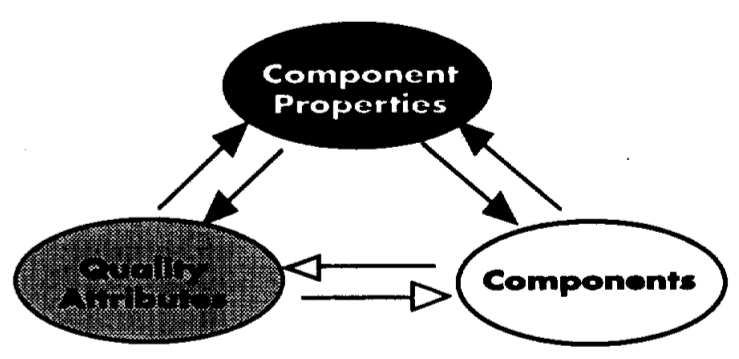
\includegraphics[width=.6\textwidth]{software-engineering/project-management/product/dromey/dromey-generic_model}
	\end{block:fact}
\end{frame}



\begin{frame}[hasnext=true, hasprev=true]
	\frametitle{Dromey}
	\framesubtitle{Structural form}

	\begin{block:fact}{Structural form}
		\begin{itemize}
			\item Estabelecido pela sintaxe da linguagem (no caso do estudo, linguagem
			de programação)
		\end{itemize}
	\end{block:fact}
	
	\begin{block:fact}{Structural forms: processos e dados}
		\centering
		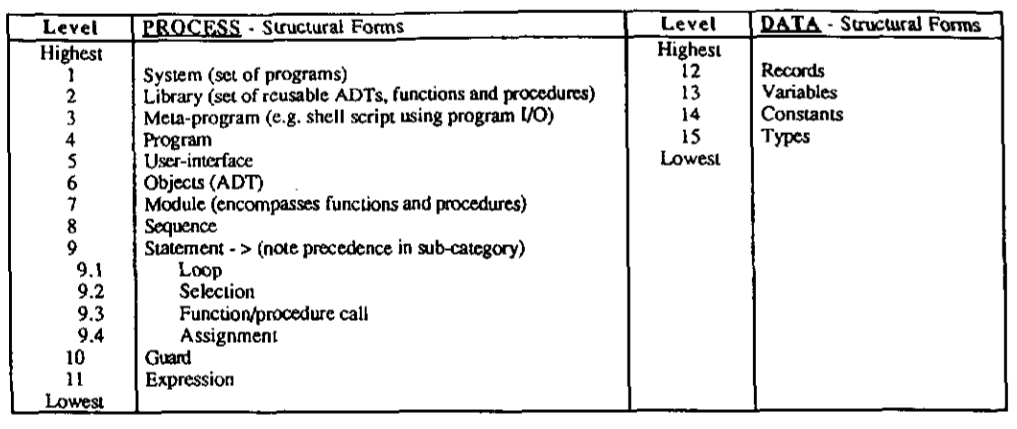
\includegraphics[width=\textwidth]{software-engineering/project-management/product/dromey/dromey-structural_forms}
	\end{block:fact}
\end{frame}



\begin{frame}
	\frametitle{Dromey}
	\framesubtitle{Atributos de qualidade}
	
	\begin{block:fact}{Atributos de qualidade}
		\begin{itemize}
			\item Funcionalidade
			\item Confiabilidade
			\item Usabilidade
			\item Eficiência
			\item Manutenibilidade
			\item Portabilidade
			\item \textbf{Reusabilidade}
		\end{itemize}
	\end{block:fact}
	
	\note{
		Os seis primeiros advém da ISO 9126.
	}
\end{frame}


\begin{frame}
	\frametitle{Dromey}
	\framesubtitle{Propriedades de qualidade}
	
	\begin{block:fact}{Atributos de qualidade e suas propriedades}
		\begin{itemize}
			\item Cada atributo está relacionado com uma ou mais propriedades de qualidade.
			
			\item Tipos de propriedades (em prioridade):
			\begin{itemize}
				\item Correção
				\item Estrutura
				\item Modularidade
				\item Descriptividade/Descrição
			\end{itemize}
		\end{itemize}
	\end{block:fact}

	\note{
		Critério para a definição das propriedades dentro de cada categoria:
		\begin{itemize}
			\item ortogonalidade,
			\item consistência,
			\item completude.
		\end{itemize}
	}
\end{frame}


\begin{frame}
	\frametitle{Dromey}
	\framesubtitle{Exemplo}

	\begin{block:fact}{Propriedade: Correctness (C1: Computable)}
		\centering
		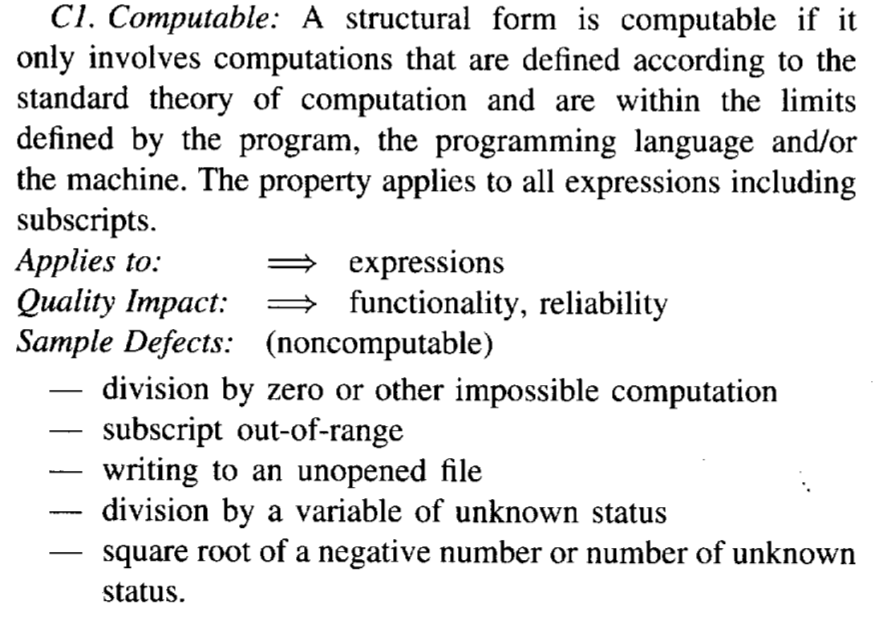
\includegraphics[width=.7\textwidth]{software-engineering/project-management/product/dromey/dromey-property_example}
	\end{block:fact}

\end{frame}



\begin{frame}
	\frametitle{Dromey}
	\framesubtitle{Propriedades de qualidade}
	
	\begin{block:fact}{Structural forms e propriedades dos atributos de qualidade}
		\begin{itemize}
			\item Cada \foreign{structural form} está relacionado com uma ou mais
			propriedades de qualidade
		\end{itemize}
	\end{block:fact}
\end{frame}


\begin{frame}
	\frametitle{Dromey}
	\framesubtitle{Propriedades de qualidade}
	
	\begin{block:fact}{Structural forms e propriedades dos atributos de qualidade}
		\centering
		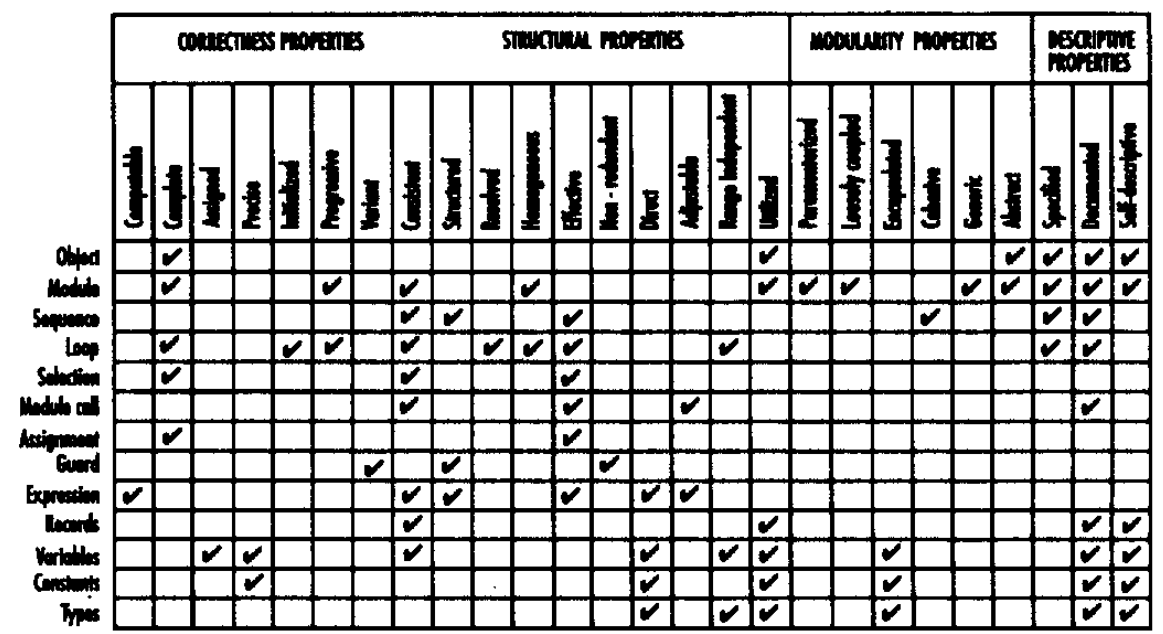
\includegraphics[width=\textwidth]{software-engineering/project-management/product/dromey/dromey-structural_forms_X_properties}
	\end{block:fact}
\end{frame}


\begin{frame}
	\frametitle{Dromey}
	\framesubtitle{Propriedades de qualidade}
	
 	\begin{block:fact}{Propriedades dos atributos de qualidade e fatores de qualidade}
		\centering
		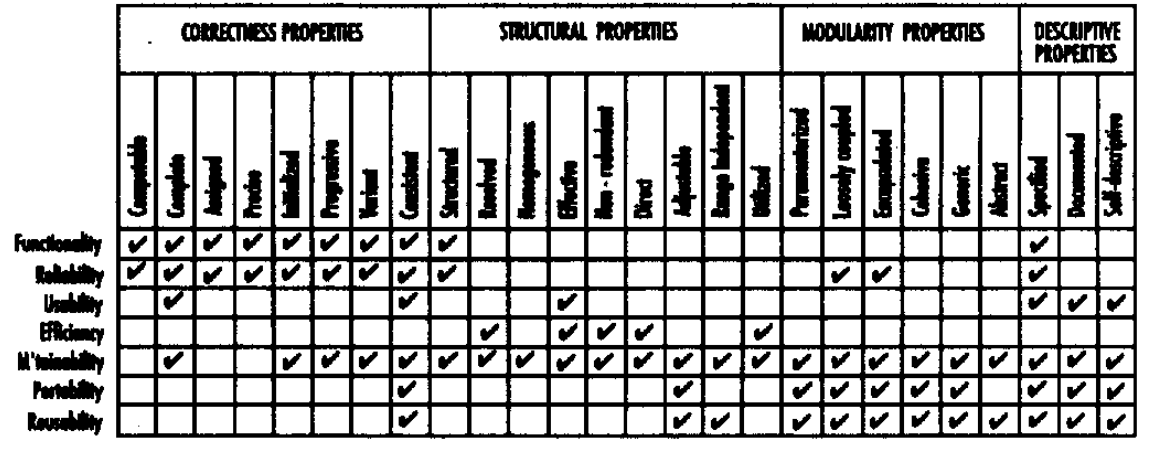
\includegraphics[width=\textwidth]{software-engineering/project-management/product/dromey/dromey-properties_X_quality}
	\end{block:fact}
\end{frame}



\begin{frame}
	\frametitle{Dromey}
	
	\begin{block:fact}{Considerações finais}
		\begin{itemize}
			\item Passível de automatização
			
			\item Não é apenas um modelo, mas um método para definir um modelo
			\begin{itemize}
				\item Identifica defeitos de qualidade, defina uma nova propriedade
				relacionada a um \foreign{structural form}
			\end{itemize}
			
			\item Não avalia diretamente a qualidade em uso
		\end{itemize}
	\end{block:fact}
\end{frame}



\subsubsection{ISO 25000}
\begin{frame}[parent={ie:agenda}, hasnext=false, hasprev=false]
	\frametitle{ISO 25000 - SQuaRE}

	\begin{block:concept}{SQuaRE}
		A série de normas 25000 ou SQuaRE (Systems and Software Quality Requirements
		and Evaluation) trata dos requisitos para planejamento e gerenciamento de
		requisitos associados aos requisitos e avaliação da qualidade de produtos
		de software.
	\end{block:concept}

	\begin{block:fact}{Quem ela substitui?}
		Aposenta a série de normas ISO/IEC 9126 e 14598.
	\end{block:fact}
	
	\begin{block:fact}{Com quem ela é compatível?}
		Processos técnicos relacionados a definição e análise de requisitos de
		qualidade das normas ISO/IEC 15288:2008 e 12207:2008.
	\end{block:fact}
		
	\note{
		\begin{itemize}
			\item ISO/IEC 15288:2008: Systems and software engineering -- System life cycle processes
			\item ISO/IEC 12207:2008: Systems and software engineering -- Software life cycle processes
		\end{itemize}
	}
\end{frame}


\begin{frame}[hasnext=true, hasprev=true]
	\frametitle{ISO 25000 - SQuaRE}

	\begin{block:fact}{Partes}
% % 		\begin{itemize}
% % 			\item ISO/IEC 2500n, Quality Management Division,
% % 			\item ISO/IEC 2501n, Quality Model Division,
% % 			\item ISO/IEC 2502n, Quality Measurement Division,
% % 			\item ISO/IEC 2503n, Quality Requirements Division,
% % 			\item ISO/IEC 2504n, Quality Evaluation Division.
% % 		\end{itemize}
		\centering
		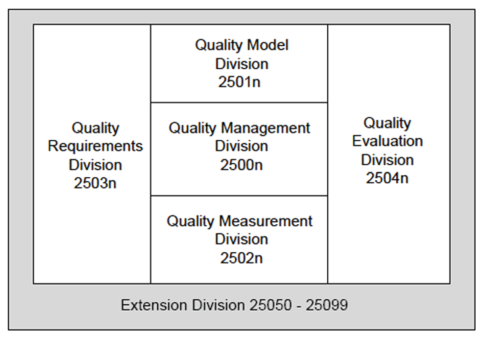
\includegraphics[width=.8\textwidth]{software-engineering/project-management/product/square}
	\end{block:fact}
\end{frame}



\begin{frame}
	\frametitle{ISO 2500n}

	\begin{block:concept}{ISO 2500n -- Gerenciamento de qualidade}
		\begin{itemize}
			\item Define modelos, termos e definições aplicáveis a todas as partes da série
			SQuaRE.
			
			\item Estabelece requisitos e diretivas para o planejamento e gestão
			associados aos requisitos e avaliação de qualidade de produto de software.
		\end{itemize}
	\end{block:concept}
	
	\begin{block:fact}{Documentos disponíveis}
		\begin{itemize}
			\item ISO/IEC 25000:2014 -- Guide to SQuaRE
		\end{itemize} 
	\end{block:fact}

	\note{
		Esta norma fornece requisitos e recomendações para uma organização responsável:
		\begin{itemize}
			\item por implementar e gerenciar a especificação de requisitos de qualidade
			do produto de software, e
			\item pelas atividades de avaliação de qualidade de software provento 
			tecnologia, ferramentas, experiências e habilidades de gestão.
		\end{itemize}
		
		Atividades:
		\begin{itemize}
			\item Motivar e treinar as pessoas para as atividades de especificação dos
			requisitos e para as atividades de avaliação,
			\item Preparar documentos apropriados,
			\item Identificar ou desenvolver métodos necessários e responder questões
			relacionadas às tecnologias que sejam relevantes.
		\end{itemize}

	}
\end{frame}

\begin{frame}
	\frametitle{ISO 2501n}

	\begin{block:concept}{ISO 2501n -- Modelo de qualidade}
		\begin{itemize}
			\item Define modelos de qualidade para produto de software, para qualidade
			em uso e dados.
		\end{itemize}
	\end{block:concept}

	\begin{block:fact}{Documentos disponíveis}
		\begin{itemize}
			\item ISO/IEC 25010:2011 -- System and software quality models
		\end{itemize} 
	\end{block:fact}

	\note{
	}
\end{frame}


\begin{frame}
	\frametitle{ISO 2502n}

	\begin{block:concept}{ISO 2502n -- Medição de qualidade}
		\begin{itemize}
			\item Define modelos de referência para medir a qualidade interna, externa
			e em uso do produto de software.
		\end{itemize}
	\end{block:concept}
	
	\begin{block:fact}{Documentos disponíveis}
		\begin{itemize}
			\item ISO/IEC 25020:2007 -- Measurement reference model and guide
			\item ISO/IEC 25021:2012 --Quality measure elements
			\item ISO/IEC 25022 -- Measurement of quality in use
			\item ISO/IEC 25023 -- Measurement of system and software product quality
			\item ISO/IEC 25024 -- Measurement of data quality
		\end{itemize} 
	\end{block:fact}

	\note{
		Equivalente à ISO 9126.
		
		Normas ISO/IEC 25022, 25023 e 25024 ainda não foram publicadas.
	}
\end{frame}


\begin{frame}
	\frametitle{ISO 2503n}

	\begin{block:concept}{ISO 2503n -- Requisitos de qualidade}
		\begin{itemize}
			\item Estabelece mecanismos para especificar requisitos de qualidade.
		\end{itemize}
	\end{block:concept}

	\begin{block:fact}{Documentos disponíveis}
		\begin{itemize}
			\item ISO/IEC 25030:2007 -- Quality requirements
		\end{itemize} 
	\end{block:fact}

	
	\note{
		ISO/IEC 2503n - Quality Requirements Division helps specifying quality
		requirements. These quality requirements can be used in the process of
		quality requirements elicitation for a product to be developed or as inputs
		for an evaluation process.
		
		The requirements definition process is mapped to Stakeholder Requirements
		Definition Process in Technical Processes defined in ISO/IEC 15288:2008 and
		ISO/IEC 12207:2008.
	}
\end{frame}


\begin{frame}
	\frametitle{ISO 2504n}

	\begin{block:concept}{ISO 2504n -- Avaliação de qualidade}
		\begin{itemize}
			\item Estabelece requisitos, recomendações e diretivas para a avaliação
			de produtos.
		\end{itemize}
	\end{block:concept}
	
	\begin{block:fact}{Documentos disponíveis}
		\begin{itemize}
			\item ISO/IEC 25040:2011 -- Evaluation process
			\item ISO/IEC 25041:2012 -- Evaluation guide for developers, acquirers and
			independent evaluators
			\item ISO/IEC 25045:2010 -- Evaluation module for recoverability
		\end{itemize} 
	\end{block:fact}
	
	
	\note{
		ISO/IEC 2504n - Quality Evaluation Division provides requirements,
		recommendations and guidelines for product evaluation, whether performed by
		independent evaluators, acquirers or developers. The support for documenting
		a measure as an Evaluation Module is also presented.
	
		Substitui a ISO/IEC 14598.
	}
\end{frame}
 

 \begin{frame}
	\frametitle{ISO 2505n}

	\begin{block:concept}{ISO 2505n -- Normas complementares}
		\begin{itemize}
			\item Normas complementares às anteriores.
			\item Normas para contextos específicos de aplicação.
		\end{itemize}
	\end{block:concept}
	
	\begin{block:fact}{Documentos disponíveis}
		\begin{itemize}
			\item ISO/IEC 25051 -- Requirements for quality of Ready to Use Software
			Product (RUSP) and instructions for testing
		\end{itemize} 
	\end{block:fact}
\end{frame}
 
 
\begin{frame}
	\frametitle{ISO 25010}
	\framesubtitle{Modelo de qualidade}

	\begin{block:fact}{Modelo de qualidade}
		\begin{itemize}
			\item Organizado em:
			\begin{itemize}
				\item Características internas e externas (características de produto)
				\item Características de software em uso
			\end{itemize}
			
			\item Todas as características possuem subcaracterísticas
		\end{itemize}
	\end{block:fact}
\end{frame}

\begin{frame}
	\frametitle{ISO 25010}
	\framesubtitle{Modelo de qualidade}
	
	\begin{block:fact}{Características de produto}
			\centering
			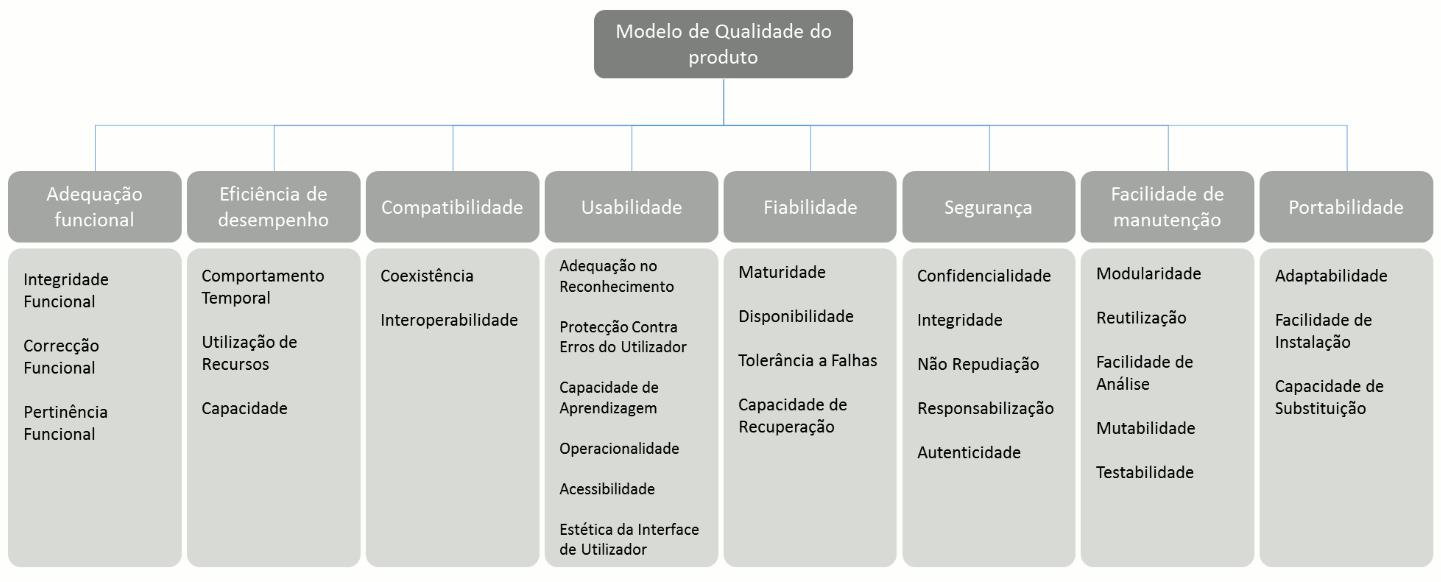
\includegraphics[width=\textwidth]{square-quality_model}
	\end{block:fact}
\end{frame}


 
\begin{frame}
	\frametitle{ISO 25010}
	\framesubtitle{Modelo de qualidade}

	\begin{block:fact}{Características de produto}
		\begin{itemize}
			\item Adequação funcional
			\item Confiabilidade
			\item Usabilidade
			\item Eficiência de desempenho
			\item \textbf{Segurança}
			\item Compatibilidade
			\item Capacidade de manutenção
			\item Portabilidade
		\end{itemize}
	\end{block:fact}
	
	\note{
		Principal mudança referente ao modelo anterior: segurança.
	
		Reflete uma necessidade e uma tendência em todos os setores da computação (vide IEEE/ACM CS 2013).	
	}
\end{frame}


\begin{frame}
	\frametitle{ISO 25010}
	\framesubtitle{Características de produto}

	\begin{block:fact}{Segurança}
		\begin{itemize}
			\item Confidencialidade
			\item Integridade
			\item Não repúdio
			\item Rastreabilidade de uso (\foreign{accountability})
			\item Autenticidade
		\end{itemize}
	\end{block:fact}
\end{frame}


 
\begin{frame}
	\frametitle{ISO 25010}
	\framesubtitle{Modelo de qualidade}

	\begin{block:fact}{Características de software em uso}
		\begin{itemize}
			\item Efetividade
			\item Eficiência
			\item Satisfação
			\item Uso sem riscos
			\item Cobertura de contexto
		\end{itemize}
	\end{block:fact}
\end{frame}

% 
%\begin{frame}
%	\frametitle{ISO 25010}
%	\framesubtitle{Características de software em uso}
%
%	\begin{block:fact}{Efetividade}
%		\begin{itemize}
%			\item Efetividade
%		\end{itemize}
%	\end{block:fact}
%\end{frame}
%
% 
%\begin{frame}
%	\frametitle{ISO 25010}
%	\framesubtitle{Características de uso}
%
%	\begin{block:fact}{Eficiência}
%		\begin{itemize}
%			\item Eficiência
%		\end{itemize}
%	\end{block:fact}
%\end{frame}
%
%
%\begin{frame}
%	\frametitle{ISO 25010}
%	\framesubtitle{Características de uso}
%
%	\begin{block:fact}{Satisfação}
%		\begin{itemize}
%			\item Utilidade
%			\item Prazer
%			\item Conforto
%			\item Confiança
%		\end{itemize}
%	\end{block:fact}
%\end{frame}
%
%\begin{frame}
%	\frametitle{ISO 25010}
%	\framesubtitle{Características de uso}
%
%	\begin{block:fact}{Uso sem riscos}
%		\begin{itemize}
%			\item Mitigação de risco econômico
%			\item Mitigação de risco a saúde e segurança
%			\item Mitigação de risco ambiental
%		\end{itemize}
%	\end{block:fact}
%\end{frame}
%
%
%\begin{frame}
%	\frametitle{ISO 25010}
%	\framesubtitle{Características de uso}
%
%	\begin{block:fact}{Cobertura de contexto}
%		\begin{itemize}
%			\item Completude de contexto
%			\item Flexibilidade
%		\end{itemize}
%	\end{block:fact}
%\end{frame}



% \subsubsection{ISO 14598}
% \begin{frame}[parent={ie:agenda}, hasnext=false, hasprev=false]
	\frametitle{Avaliação de qualidade de produto}

	\begin{block:fact}{Avaliação de qualidade de produto}
		\begin{itemize}
		 \item Repetível (pelo mesmo avaliador)
		 \item Reproduzível (por outro avaliador)
		 \item Imparcial (não ser influenciada)
		 \item Objetivo (resultados devem ser factuais)
		\end{itemize}
	\end{block:fact}
\end{frame}



\begin{frame}[hasnext=true, hasprev=true]
	\frametitle{Avaliação de qualidade de produto}
	\framesubtitle{ISO 14598}

	\begin{block:concept}{ISO 14598}
		Conjunto de normas ISO/IEC sobre a avaliação de produtos de software.
	\end{block:concept}
	
	\begin{block:fact}{Partes da norma}
		\begin{itemize}
			\item ISO/IEC 14598-1: Visão geral.
			\item ISO/IEC 14598-2: Planejamento e gestão.
			\item ISO/IEC 14598-3: Processo para desenvolvedores.
			\item ISO/IEC 14598-4: Processo para adquirentes.
			\item ISO/IEC 14598-5: Processo para avaliadores.
			\item ISO/IEC 14598-6: Documentação de módulos de avaliação.
		\end{itemize}
	\end{block:fact}
	
	\note{
		ISO/IEC 14598-2 fornece requisitos, recomendações e diretrizes para uma
		função de apoio responsável pela gestão da avaliação de produto de software
		e pelas tecnologias necessárias para a avaliação de produto de software. 
	}
\end{frame}

\begin{frame}
	\frametitle{ISO 14598-1}
	\framesubtitle{Visão geral do processo de avaliação}

	\begin{block:fact}{Fases}
		\begin{itemize}
			\item Estabelecimento de requisitos de avaliação
			\item Especificação da avaliação
			\item Projeto da avaliação
			\item Execução da avaliação
		\end{itemize}
	\end{block:fact}
\end{frame}


\begin{frame}
	\frametitle{ISO 14598-1}
	\framesubtitle{Visão geral do processo de avaliação}

	\begin{block:fact}{}
		\centering
		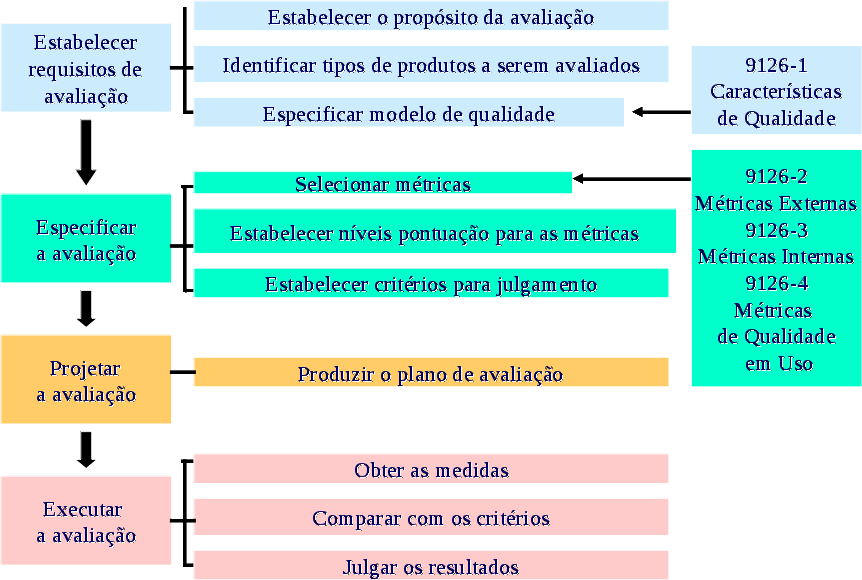
\includegraphics[width=\textwidth]{software-engineering/project-management/product/iso14598/iso14598-evaluation-process}
	\end{block:fact}
\end{frame}

%
%\begin{frame}
%	\frametitle{ISO 14598-1}
%	\framesubtitle{Requisitos de avaliação}
%
%	\begin{block:procedure}{Estabelecimento de requitos de avaliação}
%		\begin{enumerate}
%			\item Estabelecer propósito da avaliação
%			\item Identificar tipos de produtos a serem avaliados.
%			\item Especificar modelo de qualidade
%			\begin{itemize}
%				\item Por exemplo, o ISO 9126-1.
%			\end{itemize}
%		\end{enumerate}
%	\end{block:procedure}
%	
%	\note{
%		Para a fase de estabelecimento de requisitos de avaliação é necessário que 
%		tais requisitos sejam transformados em características de qualidade que
%		estão de acordo com o modelo de qualidade da ISO/IEC 9126-1. 
%		
%		Essa fase ressalta a importância dessas características  por meio da 
%		declaração do uso esperado do produto e de riscos associados.
%		
%		Dependendo do propósito da avaliação, outras normas podem ser utilizadas em
%		conjunto:
%		\begin{itemize}
%			\item ISO/IEC 14598-3: objetivo da avaliação é um produto que está sendo desenvolvido. 
%			\item ISO/IEC 14598-4: objetivo da avaliação é a compra de um produto de software no caso de processo para adquirentes
%			\item ISO/IEC 14598-5: objetivo da avaliação é a compra de um produto de software no caso de processo para avaliadores, incluindo requisitos para avaliação de terceiros.
%		\end{itemize}
%	}
%\end{frame}
%
%
%\begin{frame}
%	\frametitle{ISO 14598-1}
%	\framesubtitle{Especificação da avaliação}
%
%	\begin{block:procedure}{Especificação da avaliação}
%		\begin{enumerate}
%			\item Escolher métricas que se correlacionem com os requisitos de avaliação
%			\item Estabelecer níveis de pontuação para cada métrica
%			\item Estabelecer critérios para julgar a avaliação
%		\end{enumerate}
%	\end{block:procedure}
%	
%	\note{
%		Exemplos de métricas externas e internas apresentados na ISO/IEC 9126-2 e
%		na ISO/IEC 9126-3 podem ser aplicados nessa fase.
%	}
%\end{frame}
%
%
%\begin{frame}
%	\frametitle{ISO 14598-1}
%	\framesubtitle{Especificação da avaliação}
%
%	\begin{block:fact}{Escolha de métricas}
%		\centering
%		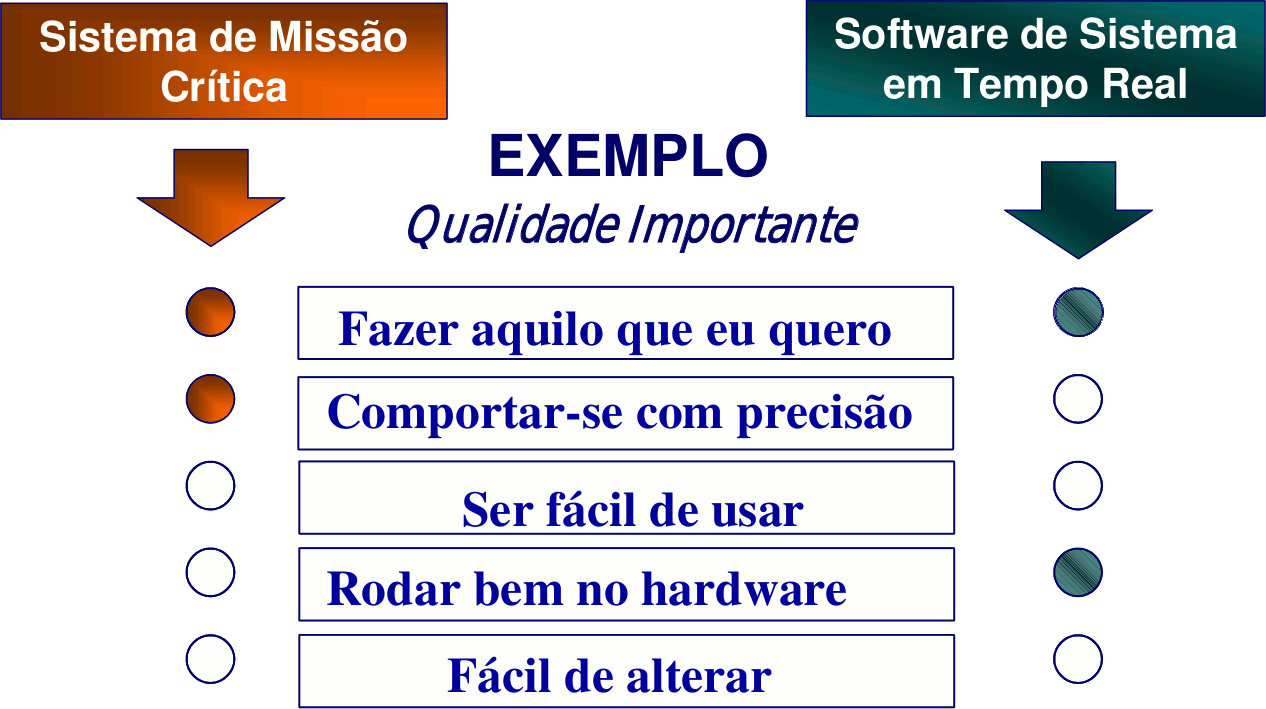
\includegraphics[width=\textwidth]{software-engineering/project-management/product/iso14598/quality-context}
%	\end{block:fact}
%\end{frame}
%
%
%
%\begin{frame}
%	\frametitle{ISO 14598-1}
%	\framesubtitle{Projeto da avaliação}
%
%	\begin{block:procedure}{Projeto da avaliação}
%		\begin{enumerate}
%			\item Documentar os procedimentos para realizar a avaliação 
%			\item Especificar os recursos necessários para executar a avaliação
%		\end{enumerate}
%	\end{block:procedure}
%	
%	\note{
%		A fase de projeto da avaliação consiste da documentação dos procedimentos
%		que serão utilizados pelo avaliador para executar a medição. 
%		
%		Os recursos necessários como, por exemplo, pessoas e técnicas, bem como a
%		sua alocação devem ser especificados para as diferentes atividades durante
%		a fase de execução da avaliação. 
%		
%		O resultado da fase de projeto da avaliação é um plano de avaliação que
%		descreve os métodos de avaliação e o cronograma das ações do avaliador. 
%	}
%\end{frame}
%
%
%\begin{frame}
%	\frametitle{ISO 14598-1}
%	\framesubtitle{Execução da avaliação}
%
%%	\begin{columns} 
%% 		\column{.4\textwidth}
%		\begin{block:procedure}{Execução da avaliação}
%			\begin{enumerate}
%				\item Coletar as medidas
%				\item Comparar com os critérios
%				\item Julgar os resultados
%			\end{enumerate}
%		\end{block:procedure}
%		
%% 		\column{.55\textwidth}
%% 		\begin{block:fact}{Escolha de métricas}
%% 			\centering
%% 			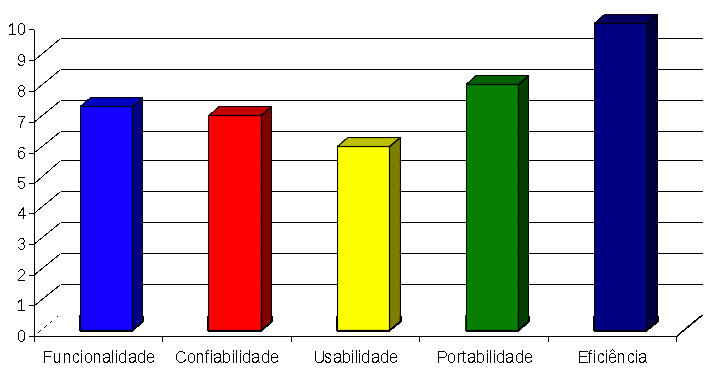
\includegraphics[width=\textwidth]{software-engineering/project-management/product/iso14598/metrics-criteria}
%% 		\end{block:fact}
%% 		\end{columns}
%		
%		\note{
%			Na fase de execução da avaliação, as métricas selecionadas são aplicadas 
%			ao produto de software, obtendo-se os valores nos níveis de pontuação. 
%			
%			Esses valores medidos são comparados com os critérios para julgamento
%			determinados anteriormente.
%		}
%\end{frame}
%
%
%
%\begin{frame}[hasnext=false, hasprev=true]
%	\frametitle{ISO 14598-1}
%	\framesubtitle{Visão geral do processo de avaliação}
%
%	\begin{block:fact}{}
%		\centering
%		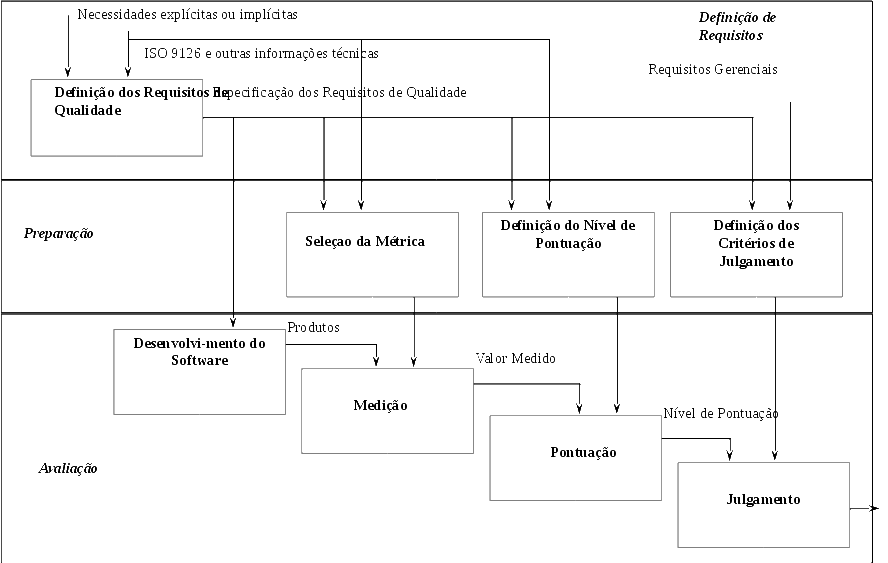
\includegraphics[width=\textwidth]{software-engineering/project-management/product/iso14598/iso14598-evaluation-process2}
%	\end{block:fact}
%\end{frame}
%
%





\backmatter{}
\part{Referências e créditos}
\part{Referências}
\section*{Referências}

\nocite{Fairley:2009}

\begin{frame}[parent={ie:agenda}, hasnext=true, hasprev=false, label=references, allowframebreaks]{\refname}
\bibliographystyle{abnt-num}
\small
\bibliography{root}
\end{frame}


\end{document}
